\section{概~~述}
要想真正理解图形接口及渲染管线,对硬件架构的一定了解是必不可少的,实际上很多3A工作室都要求图形相关的职位需要对硬件架构有一定了解。

然而,GPU的硬件架构不是一个独立的概念,它是基于CPU并行架构的发展而演变出来的,即是说理解CPU并行架构是理解GPU并行架构的重要基础;另一方面,本书同时包含离线渲染和实时渲染相关的知识,离线渲染的其中一部分是通过CPU来计算的,例如大部分光线追踪的实现,这就要求我们必须对CPU架构有一定的理解;最后,对CPU架构的了解还有助于我们编写高性能的游戏逻辑(非图形部分)代码,所以本章的内容同时包含CPU和GPU的架构知识的讨论。

通过本章的知识,读者将能对处理器的架构有比较系统的认识,并能够通过对比GPU并行架构与CPU并行架构的区别,来更好地理解GPU的特性,以帮助我们更好的学习渲染管线。




\section{CPU应用程序执行模型}\index{冯·诺依曼架构von Neumann architecture}\index[en]{von Neumann architecture冯·诺依曼架构}
几乎所有处理器都以冯·诺依曼提出的处理器结构(称为von Neumann architecture或者von Neumann model)为工作基础,冯·诺依曼被认为是计算机之父之一。在该结构中,一个具有处理单元的电子数字计算机由以下部分组成:一个用于进行二进制运算的算术逻辑单元\index{算术逻辑单元Arithmetic logic unit}\index[en]{Arithmetic logic unit算术逻辑单元}(Arithmetic logic unit,ALU),一个用来高速存储指令和数据的寄存器组\index{寄存器组processor registers}\index[en]{processor registers寄存器组}(Processor registers),一个用来控制指令读取的控制单元\index{控制单元control unit}\index[en]{control unit控制单元}(Control unit),一个用于存储所有指令和数据的内存,外加一些大容量存储设备及输入输出设备组成,如图\ref{f:rp-Neumann-Architecture}所示。

\begin{figure}
\sidecaption
	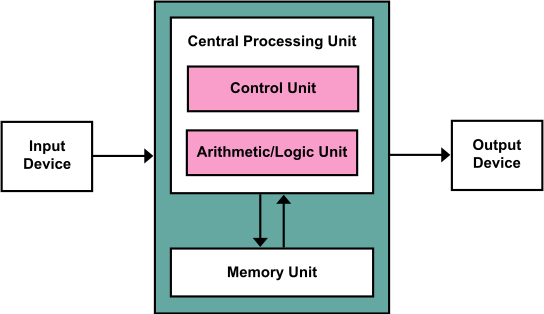
\includegraphics[width=0.65\textwidth]{figures/rp/Von-Neumann-Architecture}
	\caption{冯·诺依曼架构,图片来自Kapooht - Own work, CC BY-SA 3.0, \protect\url{https://commons.wikimedia.org/w/index.php?curid=25789639}}
	\label{f:rp-Neumann-Architecture}
\end{figure}

在冯·诺依曼模型中,处理器从内存中将指令和数据(包括地址)读取到寄存器并解码,然后执行该指令。寄存器在物理设计上靠近处理器,它是计算机所有存储设备中具有最快存取速度(通常1个CPU时钟周期)的存储设备,但是它通常只有有限的容量(几千byte),所以当寄存器中的指令或数据执行完毕后,就需要向主存读取数据。

在冯·诺依曼模型中,程序和数据存储在内存中,它们和处理器是分开的,因此数据需要在内存和处理器之间进行传输,消息传递的总时间可以用一个简单的模型来描述:一个固定的开销加上一个依赖于消息长度的可变开销,即:

\begin{equation}
	T_{message-transfer}=\alpha+ \cfrac{N}{\beta}
\end{equation}


\noindent 这个固定开销$\alpha$称为延迟\index{延迟latency}\index[en]{latency延迟}(latency),实际上它是指在通信介质上发送一条空消息所花费的时间,即从发送函数被调用到接收方完成接收数据的时间。延迟包括软件和网络硬件开销,消息在通信介质中的传输时间。带宽\index{带宽bandwidth}\index[en]{bandwidth带宽}$\beta$(bandwidth)是通信介质容量的度量,$N$表示消息的长度。

更进一步地,近年来处理器的速度得到了非常大的发展,现代处理器的运行速度通常高达4GHz;另一方面,内存的发展则主要集中在密度(即用更小的空间存储更多的数据)而不是传输速度上。所以随着处理器运行速度的提高,其花费了更多的时间用于等待从内存获取数据,不管处理器的速度多快,它都受限于内存传输速度这个瓶颈。这又称为冯·诺依曼瓶颈\index{冯·诺依曼瓶颈von Neumann bottleneck}\index[en]{von Neumann bottleneck冯·诺依曼瓶颈}(The von Neumann bottleneck)。

通常有以下以下方法用于克服冯·诺依曼瓶颈:

\begin{itemize}
	\item \emph{缓存 } 将一些频繁使用的数据存入一个特殊的更快的存储区,当处理器需要读取这些数据时可以直接从这些存储区快速读取,而不是需要从缓慢的主存读取数据。
	\item \emph{预取 } 将一些接下来可能会使用的数据在处理器读取之前放入到缓存区,以加速数据读取的速度。
	\item \emph{多线程 } 使用多线程,当其中一个线程在等待数据传输的时候切换到其他线程执行,通过是处理器保持繁忙来隐藏延迟。
\end{itemize}




\subsection{缓~~存}
几乎所有现代处理器都设计有多个层级的缓存结构以减少从主存读取数据的时间,缓存是一种容量更小,更快的内存,缓存里的数据来自于主存。当处理器需要向主存获取指令或数据时,它首先查询缓存,如果数据不在一级缓存(L1)中,则处理器向二级或三级(L2或L3)缓存发出读取请求。如果缓存中没有此数据,则需要从主存中读取。一级缓存的工作速度通常能达到或接近处理器的时钟速度,因此,假设写入和读取都是在缓存中完成,则指令的执行很有可能接近处理器全速。一级缓存的大小通常只有16KB或32KB大小,二级缓存要慢些,但空间会大些,通常约为256KB,三级缓存要大得多,通常几兆字节大小,但是比二级缓存要慢得多。如图\ref{f:rp-ps4-cache}为PS4的缓存结构。

\begin{figure}
	\sidecaption
	\includegraphics[width=0.65\textwidth]{figures/rp/cpu-cache}
	\caption{PS4分别拥有32KB的L1缓存用于存储指令和数据,L1缓存的读取速度约为3个时钟周期;2MB的L2缓存,其读取速度约为30个时钟周期;从主存读取数据则需要约220个以上的时钟周期的延迟(数据来自\cite{a:DoggedDetermination:TechnologyandProcessatNaughtyDogInc.})}
	\label{f:rp-ps4-cache}
\end{figure}

现代CPU几乎都是多核的,例如PS4\cite{a:PS4SystemArchitecture}有8个CPU内核。通常在缓存设计中,L1和L2级缓存都是每个核独享的,而L3级缓存是所有核共享的。在实际程序中,数据集(尤其是循环程序)可能非常大,以至于不能放在更高速的L1或L2缓存,这个时候即使设置了缓存,处理器仍然会因为受到内存吞吐率或带宽的限制,而无法发挥其所具有的处理能力。在\cite{a:DoggedDetermination:TechnologyandProcessatNaughtyDogInc.}中,Jason Gregory建议要保持高性能部分的程序足够小,以使其能够存储在L2级指令缓存(L1 I\$)中,同时保持高性能部分的数据足够小且相邻,使其能够存储在L1级数据缓存(L1 D\$)中。

缓存的设计实际上是利用的局部性原理(locality),包括时间局部性和空间局部性。时间局部性是指之前访问的数据很可能还要再次被访问,例如对于一个循环结构,其循环指令被多个数据使用;空间局部性是指刚刚被访问过的数据附近的数据,可能马上就会被访问,同样是循环的例子,循环的指令可能会持续访问一个数组中所有的元素。

当处理器从缓存而不是主存中取来一条指令或一个数据时,称为缓存命中\index{缓存命中cache hit}\index[en]{cache hit缓存命中}(cache hit),反之称为缓存失效(cache miss)\index{缓存失效cache miss}\index[en]{cache miss缓存失效}。缓存失效可能是由于处理器第一次访问一段新的指令或数据,这个时候它们还没有被读取到缓存中,这种情况的缓存失效可以通过下一节讲述的预取技术来解决。

第二种缓存失效的来源是缓存的尺寸限制,为此,我们需要理解缓存系统是如何从主存中读取数据的。主存载入到缓存的单位是一个缓存行(cache line)\index{缓存行cache line}\index[en]{cache line缓存行},缓存行的大小一般是64bytes,相应地缓存系统会按照最近最少使用算法(Least recently used,LRU)\index{最近最少使用算法least recently used}\index[en]{least recently used最近最少使用}替换一个旧的缓存行,这就会导致对之前缓存过的数据的访问出现缓存失效。

针对缓存系统的特定,程序员在编写程序的时候就要充分利用数据访问的局部性,例如使用顺序访问的数组。这种局部性的处理在GPU的并行计算中甚至更加重要,正如后面会讲述的关于GPU架构的内容。



缓存的设计是有代价的,例如英特尔I7-920处理器具有8MB的三级缓存,但是其占用了约$30\%$左右的芯片面积。随着缓存容量的增加,用于制造处理器的硅片的物理尺寸也逐渐变大,芯片越大,制造成本约昂贵。这使人们将注意力转向另外两种延迟隐藏\index{延迟隐藏latency hiding}\index[en]{latency hiding延迟隐藏}技术:即预取和多线程。




\subsection{预~~取}
为了减小缓存失效的几率,预取(prefetching)\index{预取prefetching}\index[en]{prefetching预取}技术就是通过在处理器读取数据之前预测可能会读取的数据,从而提前将其读取到缓存中,以进一步实现延迟的隐藏。

预取技术集成于处理器内部,各级缓存都有自己的预取器(prefetcher)\index{预取器prefetcher}\index[en]{prefetcher预取器},这些预取器是一些特定的指令用来实现数据预取,一些编译器如GCC还通过在编译阶段修改源代码,在其中插入一些预取指令以实现软件预取。

L1级缓存的预取分为指令预取(L1I\$)和数据预取(L1D\$),对于L2和L3级缓存则是将数据和指令全部存储到一起。对于数据的预取是非常复杂的,因为程序对数据的访问往往不是线性的,所以最常用的数据预取是常数步幅(constant-stride)\index{常数步幅constant-stride}\index[en]{constant-stride常数步幅}模式,即根据之前数据访问的模式(在一个常数范围内的步幅)预先载入当前数据邻近对应长度范围的数据,例如数据预取器能够预取以下例子中的数组A和B中的元素,因为其步幅为一个固定的常数:

\begin{lstlisting}[language=C++,mathescape]
for(int i = 0; i < N; i++)
    A[i*4] = B[i*3];
\end{lstlisting}

但是数据预取器则不擅长对随机数据的预测,因此如果你的程序对数据的读取在整个内存空间随机跳跃,则预取器将变得毫无用处,例如数据预取器将不能有效处理下面的程序:

\begin{lstlisting}[language=C++,mathescape]
for(int i = 0; i < N; i++)
    A[i*4] = B[rand()%N];
\end{lstlisting}

对于指令的预取,由于大部分情况下处理器按编译器编译好的顺序执行,所以程序指令数据在空间上的分布更加线性,相对数据比较简单。然而仍然有一些因素使得程序指令出现非线性化,其中第一个因素是函数指针的应用,由于处理器只有在执行指令的时候才会知道其指令是追踪一个指针,所以指令预取器对函数指针没有办法进行预处理。

另一种情况是分支预测(Branch prediction)\index{分支预测branch prediction}\index[en]{branch prediction分支预测},即当程序中出现条件语句的时候,预取器应该怎样有效地预测分支的走向呢?和数据的随机读取一样,处理器并不知道分支的走向,这个决定只有在条件被计算出来的时候才能发生,因此其不能解决延迟的问题。所以分支预测必须记录过去的历史数据,以此计算出一定的模式并对后续的分支使用该模式来预测分支走向,这就是各种不同分支预测算法的基础。

例如对于以下条件分支语句:

\begin{lstlisting}[language=C++,mathescape]
if (data[c] >= 128)
	sum += data[c];
\end{lstlisting}

这里data数组在0到255之间均匀分布,如果data数组按照升序的方式被排序过,则该循环的前半部分不会进入if条件语句,而后半部分会进入if条件语句。这个示例是非常容易预测的,因为分支沿着相同的方向重复很多次,使用一个简单的计数器就可以正确的预测分支走向(除了少数几次分支发生方向变化的地方):

\begin{fullwidth}
\begin{lstlisting}
T = branch taken
N = branch not taken

data[] = 0, 1, 2, 3, 4, ... 126, 127, 128, 129, 130, ... 250, 251, 252, ...
branch = N  N  N  N  N  ...   N    N    T    T    T  ...   T    T    T  ...

       = NNNNNNNNNNNN ... NNNNNNNTTTTTTTTT ... TTTTTTTTTT  (easy to predict)
\end{lstlisting}
\end{fullwidth}

然而,如果data数组的数据是完全随机无序的,则很难对其进行分支预测,因为我们不可能预测随机数据:

\begin{fullwidth}
\begin{lstlisting}
data[] = 226, 185, 125, 158, 198, 144, 217, 79, 202, 118,  14, 150, 177, 182, 133, ...
branch =   T,   T,   N,   T,   T,   T,   T,  N,   T,   N,   N,   T,   T,   T,   N  ...

       = TTNTTTTNTNNTTTN ...   (completely random - hard to predict)
\end{lstlisting}
\end{fullwidth}

所以对于分支条件语句,在编写程序的时候应该尽量考虑其指令的连续性,这些对处理器特性的运用会大大减少延迟,是处理器能够更有效地工作。尤其对于像光线追踪这种每帧数亿的光线计算,充分的对程序结构及数据进行优化会带来巨大的性能提升,我们将在后面的章节看到对这些知识的运用。





\section{并行计算架构}
本节我们讨论CPU并行计算的一些概念,并行计算架构的演变,由单处理器多线程架构,到多处理器架构。通过对这些架构的演变及特点的讨论,我们能够很好地了解并行计算的概念,同时最重要的,现代GPU并行计算架构正是基于这样一些技术发展而来,并且我们能够很清晰地认识到GPU并行计算与CPU并行计算的特征和区别,以使我们更好地学习后面的渲染管线。




\subsection{指令级并行}
一个简单的公式可以用于度量一个单处理器的计算性能:

\begin{equation}
	\text{指令数}/\text{秒}=\text{指令数}/\text{时钟周期}\times \text{时钟周期数}/\text{秒}
\end{equation}

\noindent 因此,对于一个单处理器,每秒钟可执行的指令数量对处理器性能的影响至关重要,本节要讨论的内容就是指令级的并行计算(Instruction-level parallelism,ILP)\index{指令级并行计算instruction-level parallelism}\index[en]{instruction-level parallelism指令级并行计算},它是指一个单处理器同时执行多条指令的能力。考虑以下串行程序:

\begin{lstlisting}
1. e = a + b
2. f = c + d
3. m = e * f
\end{lstlisting}

操作3依赖于操作1和2的结果,所以它必须等操作1和2完成之后才能执行。然后操作1和2之间并不存在依赖关系,所以它们可以被同时执行。如果我们假设以上3个操作都可以在一个周期内完成,那么全部完成3个操作的时间内2个周期,则一个周期内的指令并行数ILP值为3/2。

指令级并行技术的目标就是要尽可能地提升ILP值。通常程序员编写的程序都是串行的,其编译的指令按照一定顺序一个接着一个地执行,ILP技术 允许编译器和硬件重叠地执行多个指令,或者甚至按不同的顺序执行指令。ILP对程序员是透明的(然而我们将看到明白指令级并行的一些技术对于编写高性能程序仍有一定的指导作用),这与下一节即将讲述的单处理器多线程技术相反,后者需要程序员显式地区分可以被并行执行的线程。

由ILP的定义可知,对于相同的处理器,其ILP值是随着程序的不同而不同的,因为它跟特定程序的可并行能力有关,指令之间的依赖越少,其可并行能力越强,ILP值越高,反之则越低。硬件对串行程序执行指令级并行处理的技术有很多,本节讨论一些比较流行的ILP技术。





\subsubsection{指令管线化}
第一种是指令管线化(Instruction pipelining)\index{指令管线化instruction pipelining}\index[en]{instruction pipelining指令管线化},它也是各种ILP最重要的基础,它是指将一条指令完整的执行流程分成多个阶段(例如获取指令,解码指令,获取操作码等),每个阶段允许一条单独的指令执行。这样的划分有一些重要的原因,处理器内部针对这些特定的阶段都有专门的计算功能,如果一次只处理一条指令,那么当其中任何一个阶段发生延迟或者缓存失效等,都会导致其他功能处于等待空闲状态,不能充分利用处理器的资源。

根据实现的不同,处理器对指令处理的阶段划分也不相同,有些处理器将指令管线阶段划分为多达20,甚至30多个阶段。我们以最经典的5步划分法\footnote{\url{https://en.wikipedia.org/wiki/Classic_RISC_pipeline}}为例,这5个阶段包括:

\begin{enumerate}
	\item \emph{IF: } 获取指令(Instruction fetch)阶段,处理器从一级指令缓存L1I\$获取一个32位\footnote{如果是64位机,则指令长度为64位。}的指令,该操作通常具有1个时钟周期的延迟。在这个阶段,一个称作程序计数器(Program Counter,PC)的寄存器用来保存当前被执行指令在缓存中的地址,它被用于提供给PC预测器(PC predictor),PC预测期用这个地址直接获取指令缓冲区的一个指令,并同时将程序计数器的地址增加32位(或者64位)。这种简单的预测方式通常会在当前指令处发生分支或跳转的时候出现错误,从而导致下一次指令获取出现指令缓存失效,我们上一节讲述的指令预取技术将在这个阶段进行计算。
	
	\item \emph{ID/RF: } 解码指令以及从寄存器获取操作数( Instruction decode and register fetch)。
	\item \emph{EX: } 执行(Execute)。
	\item \emph{MEM: } 读取内存(Memory access)。
	\item \emph{WB: } Register write back
\end{enumerate}


由于将指令计算过程管线化,每个管线阶段都允许执行一条指令(每个时钟周期执行该指令的一个阶段),与工厂生产流水线的原理类似,指令管线化通过充分利用各个生产流水线,而不是需要等一个单一产品的一个阶段完成才能开始下一个阶段(导致每次除工作之外的其他流水线空闲),提高了整个管线的吞吐能力。

指令管线化得工作方式如图\ref{f:rp-5-Stage-Pipeline}所示:在第1个时钟周期,处理器读取指令1的指令;在第2个时钟周期,处理器对指令1进行解码并同时获取指令2的指令;在第3个时钟周期,处理器执行指令1,同时解码指令2以及获取指令3;以此类推,理想情况下,从第5个时钟周期开始,处理器每个时钟周期内将能同时处理5条指令。

\begin{figure}
	\sidecaption
	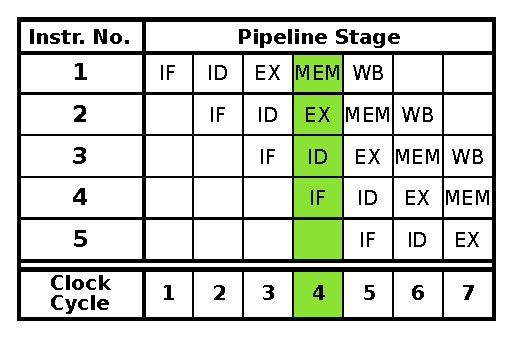
\includegraphics[width=0.5\textwidth]{figures/rp/5-Stage-Pipeline}
	\caption{指令处理的管线化,通过充分利用处理器的各个功能,管线化能够使处理器同时处理多条指令,提高了处理器的吞吐率(图片来自Cburnett)}
	\label{f:rp-5-Stage-Pipeline}
\end{figure}

然而指令管线化并不能减少延迟,当这些指令对应阶段出现延迟时(例如缓存失效,或者需要等待其他指令完成才能执行),该指令将处于停止等待状态。如果处理器每个时钟周期都能获取新的指令,处理器的利用率就能达到最大,否则这些处于等待状态的指令就会抑制对新指令的读取,降低了吞吐率。

和其他所有ILP技术一样,指令管线化的工作效率取决于应用程序的可并行性。指令管线化假设所有指令都是可以并行执行的,当程序中的指令出现依赖时,称之为一个障碍(Hazard)\index{障碍hazard}\index[en]{hazard障碍}。当然,在一般情况下,程序员不需要理会程序指令级的可并行性,而只管专注于程序逻辑编写串行代码,编译器和硬件会帮助我们队指令进行并行化以减少或避免障碍,但是编写高性能的程序则需要程序员理解这些硬件处理的方式。

通常硬件使用三种主要的方法来处理串行指令的并行障碍:

\begin{itemize}
	\item 管线气泡(Pipeline bubble)\index{管线气泡pipeline bubble}\index[en]{pipeline bubble管线气泡}
	\item 操作数前移(Operand forwarding)\index{操作数前移operand forwarding}\index[en]{operand forwarding操作数前移}
	\item 乱序执行(Out-of-order execution)\index{乱序执行out-of-order execution}\index[en]{out-of-order execution乱序执行}
\end{itemize}




\paragraph{管线气泡}
管线气泡是最简单的一种处理方式,当指令包含有障碍时,其将在解码阶段被识别,同时处理器会创建一个气泡占据该指令的解码阶段,使当前管线的解码阶段处于空闲等待状态,管线气泡将导致后续一个或多个指令被延迟。

如图\ref{f:rp-pipeline-bubble}所示,在第3个时钟周期时,紫色指令在解码阶段发现障碍同时创建气泡暂停该阶段,这里紫色指令可能需要依赖于绿色指令的输出值,气泡的出现导致后续的蓝色和红色指令被延迟一个时钟周期;在第4个时钟周期,绿色的指令可以继续前进,并产生输出值,使得紫色指令可以解码继续前进,然而此时指令管线中并没有指令进入执行阶段,以此类推,使得气泡沿管线指令方向前进,直至被挤出指令管线。在这种解决方案中,每个气泡表示该时钟周期有一个阶段处理空闲状态。

\begin{figure}
\sidecaption
	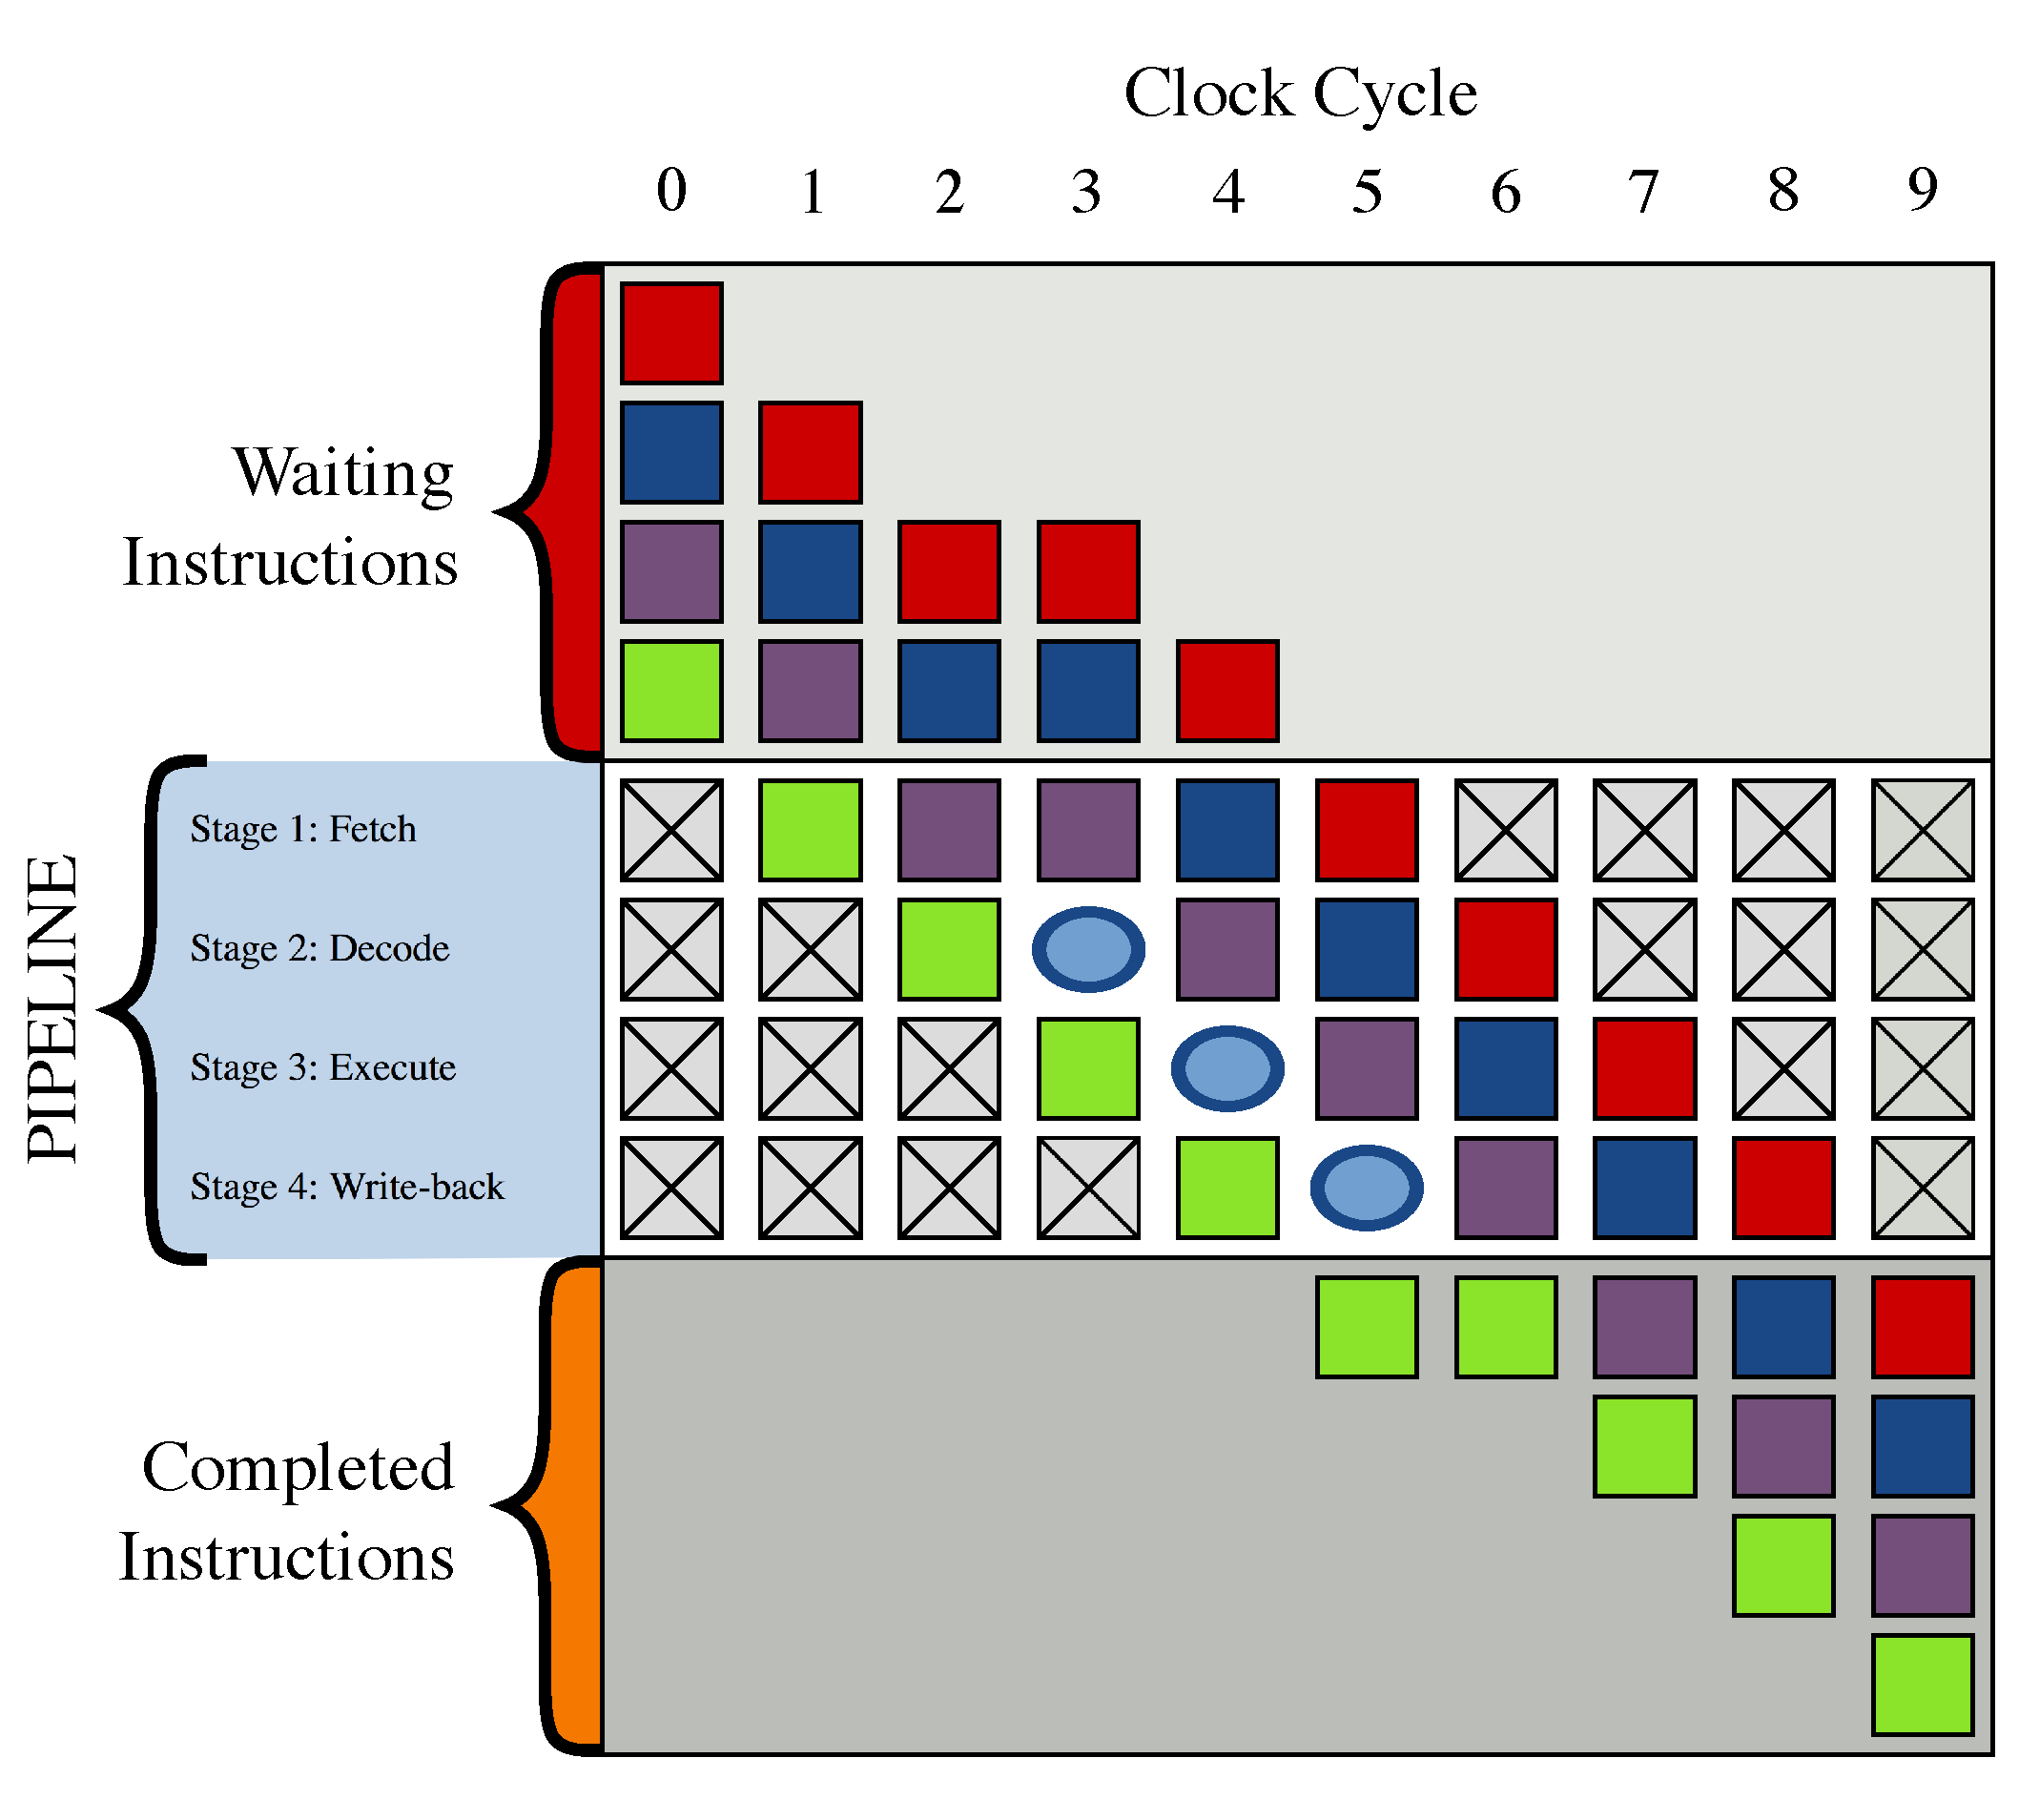
\includegraphics[width=0.65\textwidth]{figures/rp/Pipeline-bubble}
	\caption{管线气泡法在指令遇到障碍是创建一个气泡是阶段处于等待状态,知道其相应条件满足指令才才继续前进,由于气泡导致下一个时钟周期的下一个阶段没有指令可执行,因此气泡必须沿着指令管线方向前进直至被挤出指令管线(图片来自Cburnett)}
	\label{f:rp-pipeline-bubble}
\end{figure}




\paragraph{操作数前移}
当出现指令间的依赖关系时,后面的指令必须等待前面的指令执行完毕并将数据输出寄存器,后面的指令才能继续往下执行,数据写入以及从寄存器读取的过程可能占据几个时钟周期,所以上述的气泡在指令管线中停留的时间可能大于3个时钟周期以上。考虑如下两条指令:

\begin{lstlisting}
1. ADD A B C  #A=B+C
2. SUB D C A  #D=C-A
\end{lstlisting}

由于指令2中操作数A的值依赖于指令1的输出,如果指令管线每个阶段只占据1个时钟周期,则这两条指令的执行将导致指令2被延迟3个周期,如下表所示(也可以从图\ref{f:rp-pipeline-bubble}看出这种关系):

\begin{table}
\caption{在经典的5步指令管线划分法中,前后相邻且在每个阶段占据1个时钟周期的假设下,指令2将被延迟3个时钟周期}
\label{t:rp-pipeline-bubble}

\begin{tabular}{p{0.09\textwidth}|p{0.09\textwidth}|p{0.09\textwidth}|p{0.09\textwidth}|p{0.09\textwidth}|p{0.09\textwidth}|p{0.09\textwidth}|p{0.09\textwidth}|p{0.09\textwidth}|p{0.09\textwidth}}
\hline 
   指令&1&2&3&4&5&6&7&8&9  \\
    \hline  
 1&IF&ID&EX&MEM&WB&&&&\\
 2&&IF&stall&stall&stall&ID&EX&MEM&WB\\
 \hline 
\end{tabular}
\end{table}

观察表\ref{t:rp-pipeline-bubble},指令2的ID阶段和指令1的EX阶段处于同一个时钟周期,如果能够在芯片集成电路内部直接将指令1的值传递给指令2,而直接绕开寄存器,那么其将能够直接避免掉这种前后依赖关系导致的障碍。操作数前移正是基于此原理用来克服指令障碍的方法方法,在操作数前移方法中,处理器需要对指令探测这种依赖性的存在,然后根据探测结果判断是需要从寄存器中获取操作数,还是直接通过相关的电路直接获取前一指令的值。操作数前移的操作如表\ref{t:rp-operand-forwarding}所示。由于程序中通常存在大量这种前后依赖关系,操作数前移技术不仅能够有效避免这种障碍,而且大大节省了数据在寄存器之间存储和读取导致的时间延迟。

\begin{table}
\caption{在操作数前移技术中,如果处理器探测到依赖性的存在,则直接将前一指令计算的结果传递给后面的指令,避免了气泡导致的延迟}
\label{t:rp-operand-forwarding}

\begin{tabular}{p{0.09\textwidth}|p{0.09\textwidth}|p{0.09\textwidth}|p{0.09\textwidth}|p{0.09\textwidth}|p{0.09\textwidth}|p{0.09\textwidth}|p{0.09\textwidth}|p{0.09\textwidth}|p{0.09\textwidth}}
\hline 
   指令&1&2&3&4&5&6&7&8&9  \\
    \hline  
 1&IF&ID&EX&MEM&WB&&&&\\
 2&&IF&ID&EX&MEM&WB&&&\\
 \hline 
\end{tabular}
\end{table}



\paragraph{乱序执行}
乱序执行(Out-of-order execution,OoOE)\index{乱序执行out-of-order execution}\index[en]{out-of-order execution乱序执行}技术基于这样一个事实,即如果后面的指令不依赖于前面的指令,或者说它此时具备执行指令需要的操作数数据,则它可以先于前面的指令被执行。这种顺序的调整导致其程序指令被执行的顺序(称为数据顺序,data order)跟程序本身被编写的串行顺序(称为程序顺序,program order)可能不一样。

尽管指令被执行的顺序发生了改变,然而乱序执行必须保证指令执行结果输出的顺序与程序顺序保持一致,以保证最终程序运行的正确性。乱序执行的指令执行步骤如下:

\begin{enumerate}
	\item 获取指令。
	\item 将指令分配到一个指令队列。
	\item 指令在指令队列等待,直到其输入操作数可用,此时它可以早于自己前面的指令被执行。  
	\item 执行指令。
	\item 将指令输出结果保存在一个队列中。 
	\item 只有当一个指令的之前所有指令被执行完毕,并且其结果被写入到寄存器之后,才将该指令的结果输出到寄存器,以保证执行结果的顺序一致。
\end{enumerate}




\paragraph{分支预测对指令管线的影响}
除了指令间的依赖关系,前面讲述的分支预测也可能会对指令管线的性能有比较大的影响,考虑如图\ref{f:rp-mispredict}所示的分支语句,程序执行时正确的分支流向为AEFG,我们来分析如果分支预测器预测的结果为ABCD会发生什么情况。

\begin{figure}
	\begin{subfigure}[b]{0.382\textwidth}
		\includegraphics[width=1.\textwidth]{figures/rp/mispredict}
	\end{subfigure}
	\begin{subfigure}[b]{0.6\textwidth}
		\includegraphics[width=1.\textwidth]{figures/rp/mispredict-2}
	\end{subfigure}
\caption{分支预测失败会导致处理器放弃并销毁之前所有未执行完且判断错误的分支指令(图片来自\cite{a:DoggedDetermination:TechnologyandProcessatNaughtyDogInc.})}
\label{f:rp-mispredict}
\end{figure}

由于分支的真实走向必须等到if比较指令执行完毕,并且将结果写入到寄存器之后,处理器才会知道真正的分支走向。在这个例子中,即是必须等到A指令执行完毕,在A指令的第4个时钟周期之前,B,C及D指令会依次被执行,等到第4个时钟周期A指令计算完毕之后,在第5个时钟周期开始,处理器将重新将正确的EFG指令载入执行单元执行指令计算,同时销毁之前所有关于BCD在寄存器中的数据及其他相关状态。这种代价在指令管线的阶段划分越多时越严重,因为有更多不应该被执行的指令被执行了一部分,之后整个状态还需要被重置。

此外,如果if比较函数是对两个浮点数进行比较,则代价更高。浮点数比整数的比较要花费更多的时钟周期,这会导致那些被错误执行的指令被执行更多的指令阶段,从而造成处理器资源的更大浪费。

由于条件分支导致处理器资源浪费,现代处理器大都采用一种方法来避免比较和跳转操作,从而能够减轻分支带来的性能开支。这种方法基于一个第三个参数,来在两个操作数之间进行选择,而不需要执行比较和跳转指令,这种方法称为条件转移(conditional move)\index{条件转移conditional move}\index[en]{conditional move条件转移}或者无分支选择(branchless select)\index{无分支选择branchless select}\index[en]{branchless select无分支选择}。

条件转移类似于C++中的三元操作符,在处理器中,一个浮点数条件转移操作符称作fsel,它具有如下的指令形式:

\begin{lstlisting}
fsel f0, f1, f2, f3 // f0 = ( f1 >= 0 ? f2 : f3 )
\end{lstlisting}

编译器往往能够将三元操作符直接转换为fsel操作符:

\begin{lstlisting}
	return a >= 0 ? b : c;	-->   fsel fr1,fr1,fr2,fr3
\end{lstlisting}

甚至如:

\begin{lstlisting}
// float a, b, c, d, e, f;
return ( a >= 0 ? b + 1 : c + 2 ) + ( d >= 0 ? e + 1 : f + 2 ) ;
\end{lstlisting}
也可以转换为:

\begin{lstlisting}
fr1 = a, fr2 = b, fr3 = c,
fr4 = d, fr5 = e, fr6 = f
fr0 = 1.0, fr13 = 2.0f
fadds   fr12,fr2,fr0      ; fr12 = a + 1
fadds   fr11,fr3,fr13     ; fr11 = c + 2
fadds   fr10,fr5,fr0      ; fr10 = e + 1
fadds   fr9,fr6,fr13      ; fr9  = f + 2
fsel    fr8,fr1,fr12,fr11 ; fr8  = a >= 0 ? fr12 : fr11
fsel    fr7,fr4,fr10,fr9  ; fr7  = d >= 0 ? fr10 : fr9
fadds   fr1,fr8,fr7     ; return = fr8 + fr7
\end{lstlisting}

通过上面的示例可以看出,fsel对两个输入值都需要进行计算,即相当于计算了原来if条件语句的两个分支语句。然而即便如此,fsel带来的性能提升仍然十分明显,尤其是当程序中有大量if条件语句并列,或者在一个循环语句中穿插if条件语句等情形,这些带来的处理器资源浪费极大。在\cite{a:DoggedDetermination:TechnologyandProcessatNaughtyDogInc.}中,Jason Gregory建议对于高性能部分,尽量使用fsel指令,并且拆分循环内的条件语句,尽可能地使用简单的,少分支的算法。






\subsection{线程级并行}
上一节我们介绍了指令级的并行技术,这些技术大都通过硬件来实现,其中编译器能够针对这些硬件实现进行一定的优化,但是它们对于程序员而言一般是透明的。此外,指令级的并行技术还包括其他很多比较流行的技术实现,我们所讨论的几乎都是能够对编写代码具有一定指导意义的技术,这能够帮助我们编写更高性能的代码,毕竟实时的游戏程序对性能有着贪婪的要求。

在计算机科学中,一个最小单元的,可以独立被处理器调用的指令的集合称为一个线程(thread),在前面讨论的指令级并行技术中,在处理器中执行的一个单独的程序即可以称为一个单线程。在单个处理器内部,即使使用前面讲述的指令并行技术,只同时执行单个线程的处理器的利用率通常仍然很低,其原因是某些操作需要很长时间的延迟,例如数据密集型的程序需要加载大量的数据,或者线程需要等待外部的输入事件或者其他系统事件。为了进一步提高单个处理器的计算性能,多线程技术应运而生。

多线程技术(Multithreading)是指在单个处理器或者一个多核处理器的其中一个核内部,拥有同时执行多个线程的能力,它区别于后面即将讲述的多处理器架构,这些线程在内部共享该处理器的各种资源,包括计算单元,寄存器,缓存等。

在现代操作系统中,多线程技术是直接被操作系统支持的。不同于指令级并行是对用户透明的,为了充分利用多线程技术,程序员需要将一个程序中可以独立并行执行的部分拆分成单独的线程,然后操作系统根据一定的规则控制和调度处理器执行这些线程。如图\ref{f:rp-multithreading}所示,每个应用程序可以拥有一个或多个线程,其中至少一个主线程(Primary thread),以及零个或多个次级线程(Secondary thread),每个线程被赋予一定的优先级,这些线程被放入到一个线程池,操作系统以线程为单位将这些程序指令发送到处理器进行执行,其调度的方式通常是基于时间片。

\begin{figure}
	\sidecaption
	\includegraphics[width=0.45\textwidth]{figures/rp/multithreading}
	\caption{多个线程可以在一个单独的处理器上执行,每个应用程序可以创建一个或多个线,这些线程并被操作系统按照一定的优先级调用处理器进行处理}
	\label{f:rp-multithreading}
\end{figure}

如图\ref{f:rp-multithreading}所示,多线程处理器内部可以支持多个线程并行执行,但是这些线程不是真正地同时执行,而是通过处理器的控制交叉地执行。当当前正在执行的线程遇到缓存失效或者其他事件(例如一个线程需要等待另一个线程的输出结果)时,处理器即自动切换到其他处于等待执行状态(ready to run)\index{等待执行状态ready to run}\index[en]{ready to run等待执行状态}的线程(即数据已经加载到缓存)执行指令,通过这样保持处理器的繁忙,避免处理器等待数据从主存读取的延迟,来充分提高单个处理器的计算性能。

使用硬件对多线程技术的支持的一个目标是,允许在等待延迟的线程和已经准备好被执行的线程之间保持快速切换,为了达到这个目标,每个线程都需要拥有自己的指令和数据寄存器集合,还包括用于存储指令管线调度相关的一些处理单元和调度信息,当发生线程切换时,直接在高速的寄存器之间就行赋值和读取即可,而不需要重新从缓存读取数据。现代处理器的线程切换通常可以在一个时钟周期内完成。

单处理器多线程技术的这些核心思路,主要包括始终切换到处于“准备好”的状态的线程,以及使用更多专有的寄存器来实现线程之间的快速切换,被用于后来的GPU架构中,当然GPU会有一些自己独特的“思维”,但是其核心架构都是随着CPU并行计算的发展而演变出来的,再结合下一节的多处理器技术,我们就可以推导出一个可以具有无限扩展,并且能够高效利用每个GPU处理器计算单元的并行计算模型。




\subsubsection{同时多线程技术}
多线程技术有多种实现方案,最简单的是Block multithreading,这种方案会一直执行一个线程,直至线程遇到很大的延迟(例如缓存失效,这种延迟可能需要上百个时钟周期)时切换到另一个处于“可执行状态”的线程。

另一种比较聪明的方案称为交叉多线程(Interleaved multithreading)\index{交叉多线程interleaved multithreading}\index[en]{interleaved multithreading交叉多线程},这种技术在每个时钟周期都使用一个不同于上一个时钟周期的线程。由前面的内容可知,当处理器在执行一个线程时,指令级并行会使得该线程内多条指令可以被同时执行,这主要通过指令管线来实现,然而指令之间常常由数据依赖关系,而使得后面的指令在管线中使用气泡填充,虽然有一些指令级的技术用于减少气泡的占用时间,交叉多线程则试图通过线程级的技术来解决这个问题。因为线程之间是相对独立的,所以交叉多线程每次从不同的线程中取出一条指令加入到指令管线中,这样理想的情况下指令管线中每个阶段执行的是不同线程中的指令\footnote{这里可能比较费解,回想前面讲述的指令管线知识,虽然每个时钟周期内每个管线阶段执行的是不同的指令,但是每个时钟周期处理器只加入一条指令,所以如果每个时钟周期取来不同线程的指令,那么管线各个阶段执行的将是来自不同线程的指令。},从而几乎不会有数据依赖光线。然而交叉多线程的不足是每个指令阶段都需要额外的计算和存储成本用来追踪这些线程的ID。

上述两种方案都可以称为时分多线程技术(temporal multithreading,TMT)\index{时分多线程技术temporal multithreading}\index[en]{temporal multithreading时分多线程技术}技术,在TMT中,给定的任何时间对于指令管线的每个阶段只有一个线程的指令在执行,如图\ref{f:rp-smt}左边的架构。本节我们主要要讲述的,也是现代处理器比较高级的多线程技术方案是同时多线程技术(Simultaneous multithreading,SMT)\index{同时多线程技术simultaneous multithreading}\index[en]{simultaneous multithreading同时多线程技术},与TMT相对应,在一个给定时间内及指令阶段,SMT处理器可以同时有来自多个线程的指令在执行,如图\ref{f:rp-smt}右边的架构。SMT并不需要对普通的TMT架构做太大改变,它只需要增加在一个时钟周期内从多个线程获取指令的能力,以及更大的寄存器文件用于存储多个线程指令的相关数据。SMT并发线程的数量由芯片设计者决定,通常的设计为每个处理器2个并发线程,但是一些处理器支持8个并发线程。

\begin{figure}
	\includegraphics[width=0.9\textwidth]{figures/rp/smt}
	\caption{两种经典的多线程架构,左边为TMT,右边为SMT,SMT在每个时钟周期的每个阶段内,可以同时执行来自多个线程的指令。从图中可以看出,理论上SMT执行相同数量的指令只需要花费TMT一半的时钟周期}
	\label{f:rp-smt}
\end{figure}


SMT与诸如英特尔的双核处理器是不同的,虽然它们最终都是集成在一个芯片上,但是双核处理器拥有独立的执行单元,指令调度,寄存器,L1缓存等,它们只是共享L2及以上的缓存,我们可以称之为缓存级别的共享;而SMT则是共享指令级的一些资源,接下来将讲述这些共享的资源,通过共享这些指令级的资源,我们看到SMT可以大大提升单个处理器的执行效率。

我们将以英特尔的超线程技术来分析同时多线程技术,英特尔的超线程技术(Hyper-Threading Technology)\index{超线程技术hyper-threading technology}\index[en]{hyper-threading technology超线程技术}是一种SMT架构,在结构上,一个超线程架构的处理器由两个逻辑处理器(logical processor)\index{逻辑处理器logical processor}\index[en]{logical processor逻辑处理器}组成,每个逻辑处理器拥有自己的如架构状态等,但是两个逻辑处理器共享处理器的一些执行资源(Processor Execution Resources),如图\ref{f:rp-hyper-threading}所示。

\begin{figure}
	\includegraphics[width=1.\textwidth]{figures/rp/hyper-threading}
	\caption{在英特尔的超线程技术架构中,每个物理处理器包含两个逻辑处理器,每个逻辑处理器包含独立的处理器架构状态,两个逻辑处理器共享除架构状态之外的所有处理器资源。注意图中的计算机是包含两个物理处理器的,或者为后面讲述的双核处理器}
	\label{f:rp-hyper-threading}
\end{figure}

每个逻辑处理器拥有的资源包括:

\begin{itemize}
	\item 拥有独立的架构状态(Architectural State)\index{架构状态architectural state}\index[en]{architectural state架构状态}
	\item 并发地执行自己的指令
	\item 正在执行的指令可以被独立地打断和停止
\end{itemize}

两个逻辑处理器共享:
\begin{itemize}
	\item 处理器执行引擎(Execution engine)\index{执行引擎execution engine}\index[en]{execution engine执行引擎}以及L1缓存
	\item 共享系统数据总线(system bus interface)\index{系统数据总线system bus interface}\index[en]{system bus interface系统数据总线}
\end{itemize}

处理器架构状态包括数据寄,控制,调试等相关的寄存器以及一些状态机相关的寄存器,此外每个逻辑处理器还独立的高级可编程打断控制器(advanced programmable interrupt controller,APIC)\index{高级可编程打断控制器advanced programmable interrupt controller}\index[en]{advanced programmable interrupt controller高级可编程打断控制器}用来控制指令的停止等操作。从一个软件的视角来看,一旦每个逻辑处理器拥有自己的处理器架构状态,它在功能上就相当于两个独立的处理器。相对于整个处理器来说,用于存储处理器架构状态的晶体管只需要很小的面积,它相对于双核处理器大大节省了芯片面积。

超线程技术复制的处理器架构状态用来跟踪程序或线程执行流相关的信息,而其共享的执行资源则包含怎样控制这些执行流的工作展开。所有逻辑处理器共享一个物理处理器除架构状态之外的所有资源,包括执行单元,分支预测,控制逻辑及系统总线等。

\cite{a:IntelHyper-ThreadingTechnology}指出,通常应用程序只利用了单个处理器35\%的执行资源,而超线程技术可以提高处理器的利用率以达到50\%的利用率。






\subsection{处理器级并行}
前面讲述的指令级并行及线程级并行都旨在提高单个物理处理器的执行效率,然而单个物理处理器的计算能力总是有限的,只有进化到处理器级的并行,即拥有能够扩展物理处理器的能力,大规模,可扩展的并行计算才有可能形成。

多处理器架构(multiprocessing architecture)\index{多处理器架构multiprocessing architecture}\index[en]{multiprocessing architecture多处理器架构}是指一个计算机系统拥有多个物理的处理器,或者拥有多个核(Core),两者的主要区别为多核处理器每个核仅拥有的L1缓存及寄存器,同一芯片内的核共享L2及主内存,而多个单独的物理处理器往往仅共享主存并拥有自己的缓存系统。


关于多处理器架构,我们可以从两个角度来了解其特点,其一是所有处理器之间的对称性,其二处理器之间的通信机制。



\subsubsection{多处理器架构的对等性}
对称性是指所有处理器的地位和功能是否对等,非对等多处理器架构(Asymmetric multiprocessing,ASMP)\index{非对等多处理器架构asymmetric multiprocessing}\index[en]{asymmetric multiprocessing非对等多处理器架构}比较典型的例子是Cell处理器架构,它的思想是用一个常规处理器作为监管处理器,该处理器与大量的高速协作处理器相连。在Cell处理器中,常规的PowerPC处理器担任与流处理器和外部世界的接口,称为PPE(Power Processor Element),而协作处理器SPE(Synergistic Processing Element)\index{协作处理器Synergistic Processing Element}\index[en]{Synergistic Processing Element协作处理器},则在PPE的管理下处理数据集,如图\ref{f:rp-cell}所示。

\begin{figure}
	\includegraphics[width=1.\textwidth]{figures/rp/cell-architecture}
	\caption{Cell系统架构,它集成一个PPE处理器和8个SPE处理单元在一个统一的系统架构中,其中PPE是一个普通的64位的Power架构的处理器用于处理一般并行任务,而SPE主要负责数据密集型的计算,所以处理器之间通过EIB相连进行高性能的数据通信,关于更多有关Cell处理器的信息,参见\cite{a:SynergisticProcessinginCellsMulticoreArchitecture}}
	\label{f:rp-cell}
\end{figure}


要想为Cell处理器编程,你需要写一个在PowerPC核心处理器上运行的程序,该程序会用一个互不相同的二进制码,在每个流处理器单元SPE上,调用执行一个程序。实际上每个SPE本身是一个核,它可以从自己的本地取出一个独立的程序来执行,这个程序与旁边的SPE执行的程序是不同的。另外,通过一个共享的互联网络EIB(Element interconnect bus),SPE之间,SPE与PowerPC核之间可以相互通信。

Cell处理器的设计目标之一是克服由于内存访问的延迟对处理器性能的制约,在那个时代的分析显示,即使高速的处理器也浪费约80\%的时间用于等待数据从内存读取。因此,即使处理器的计算速度再快,内存访问仍然是一个重要的制约因素。所以,Cell处理器的独特之处在于它摒弃了传统的内存缓存结构,而是直接将数据和指令直接发送到每个SPE处理器的一个本地私有内存空间LS(Local store)\index{本地存储local store}\index[en]{local store本地存储},SPE直接从LS存取数据,每个SPE拥有一个直接内存存取(Direct memory access,DMA)\index{直接内存存取direct memory access}\index[en]{direct memory access直接内存存取}引擎,用于将LS的数据高速同步到其他SPE或者PPE的内存。

我们对Cell架构感兴趣是因为它很像现代图形处理器的架构,这有助于我们对比和理解下一节的图形处理器。首先SPE主要聚焦于数据密集型计算,例如图像处理以及很多数学物理方面的计算(例如傅里叶变换),这些计算的并行性特征很强,所以每个SPE是完全基于SIMD的数据结构,它简化了寄存器设计,没有像常规处理器一样用于如整数,浮点数指令的各种寄存器类型(整型,单/双精度浮点型,布尔类型,以及地址),它只有一个128为的SIMD寄存器,并用来存储各种数据类型,这些数据类型完全没有针对硬件的特征\footnote{例如数据类型在不同处理器上的长度不一致将导致处理器的指令解码等操作需要做一些额外的工作。},这和现代GPU的设计是一致的。这简化了处理器的设计,使得编译器对寄存器的分配也简化了很多,同时大大节省了芯片面积,使同样的芯片面积可以扩展更多的SPE处理器。

另一个和GPU很像的特征是,它并且了常规处理器的多级缓存系统,而是直接将数据从主存通过DMA高速读取到LS,为了更有效的工作,你需要将一个计算的大量数据提前搬到SPE,让它一次性尽可能做更多的计算,而不是像缓存系统那样每次从缓存系统读取少量的数据。在处理器中,缓存系统占据了很多的芯片面积,并且导致能耗的增加。这种设计架构也能大大减少芯片面积及能耗。

Cell处理器最早被用在PS3中\cite{a:PlayStation3SystemArchitecture},然而由于它相对于传统串行编程具有一定的开发成本,并且它不支持乱序执行等特征,以及价格相对比较昂贵,PS4重新又回到了传统的x86架构。然而Cell处理器仍被用于高性能计算,以及其他数学,物理,医学等科学计算中。

对于对等多处理器(Symmetric multiprocessor,SMP)\index{对等多处理器symmetric multiprocessor}\index[en]{symmetric multiprocessor对等多处理器}架构则比较简单,更多的处理器主要是增加了并行的能力,应用程序的线程还是通过操作系统来分配,对开发者来讲,我们仅仅需要掌握针对多线程编程的知识即可。




\subsubsection{多处理架构的通信方式}
由于处理器的计算是以线程为单位的,而线程之间是会共享数据的,因此每个处理器之间需要进行通信,根据这种通信机制的不同,多处理器架构可以分为共享内存以及基于网络的消息传递方式。

在内存共享方式中,每个处理器拥有自己的缓存系统,但是它们共享整个计算系统的主内存,如图\ref{f:rp-smp}所示。基于内存共享的架构方式实现比较简单,然而由于缓存是主内存内部分数据的复制,如果同一应用程序的多个线程分布在多个缓存系统内,则需要通过某种同步机制保证各个处理器内的缓存一致性(Cache coherence)\index{缓存一致性cache coherence}\index[en]{cache coherence缓存一致性},即一个内存的写操作需要通知所有核的各个级别的缓存,因此,无论何时,所有处理器核看到的内存试图是完全一样的。随着处理器中核数量的增多,这个通知的开销迅速增大,使得缓存一致性成为限制一个处理器中核数不能太多的一个重要因素。缓存一致系统中最坏的情况是,一个写内存操作会迫使每个核的缓存都进行更新,进而每个核都要对相邻的内存单元进行写操作\footnote{回想缓存中的数据更新是以缓存行为单位的。}。

\begin{figure}
	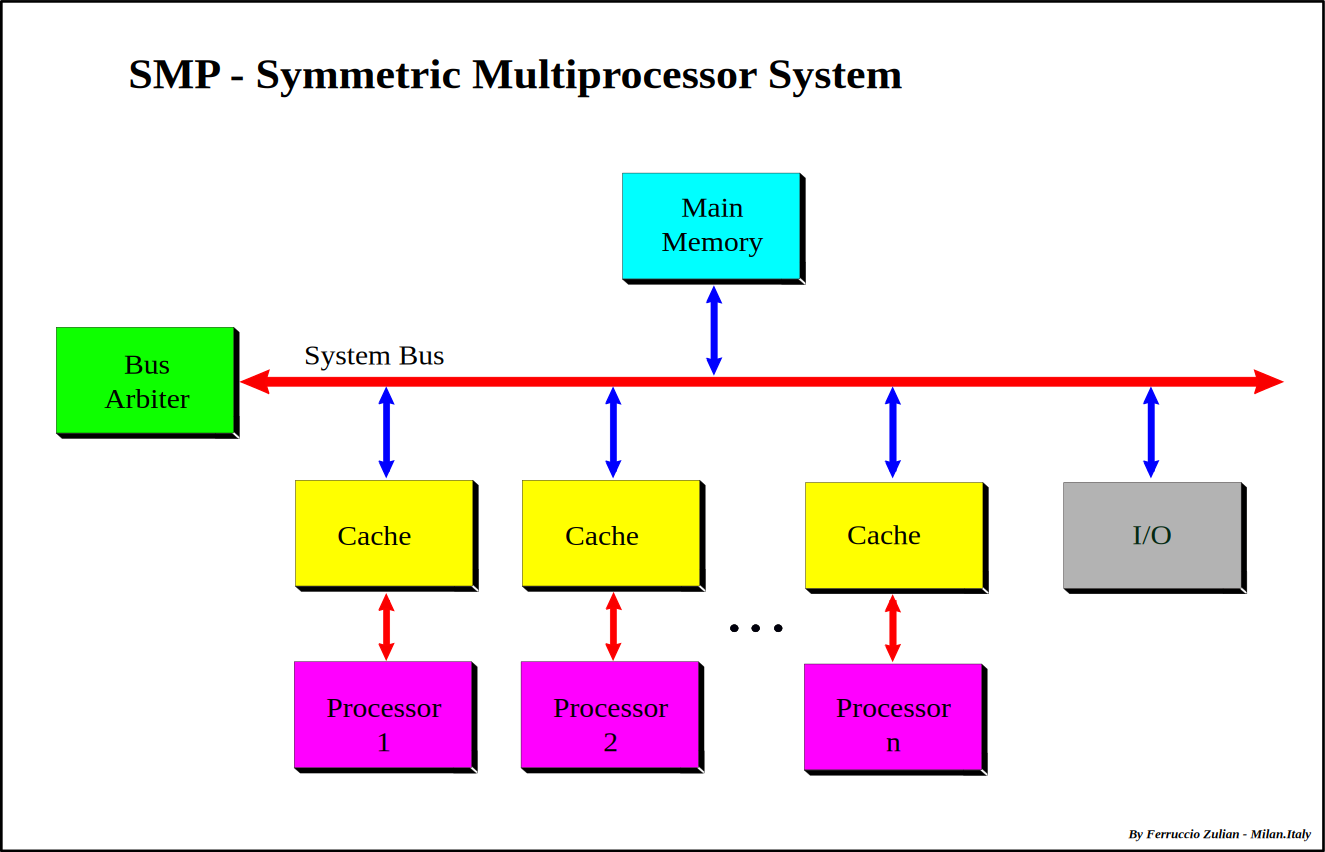
\includegraphics[width=1.\textwidth]{figures/rp/smp}
	\caption{一个共享内存的多处理器架构,每个处理器拥有独立的缓存系统,并通过系统总线共享主内存(图片来自Ferry Milan)}
	\label{f:rp-smp}
\end{figure}

另一种多处理器的架构称为集群,即通过将一些独立的通常是廉价的计算机系统,通过网络等方式联通起来,组成一个多处理器系统。集群的架构具备很高的扩展性,然而由于网络传输的速度很慢,所以处理器之间的通讯具有很大的延迟,它更适合于线程之间的耦合相对比较弱的计算,例如对一张图片的处理,可以把它分成多个部分,如果每个部分的处理是相对独立的,则可以把不同部分发送到不同的计算机上进行计算。

由于缓存一致的的代价,使得共享内存的架构并不太适合高性能的并行计算,所以我们将会看到后面的GPU架构以及前面的Cell处理器架构都是在试图避免使用缓存,来避免缓存一致性的需求。对于那些数据密集型以及高度并发性的程序,将大量数据直接发送到处理器附近的内存,以及使用大容量寄存器来达到高速存储,并且仅对本地数据进行读写操作以减少数据同步的问题,这种简化的架构使得并行计算的性能更高。




\subsubsection{弗林分类法}	
在此之前的所有对处理器架构知识的描述中,我们主要聚焦于处理器的物理结构,对于程序或者编程人员而言,我们提出使用另一种方式来描述处理器架构,即弗林分类法(Flynn's taxonomy)\index{弗林分类法Flynn's taxonomy}\index[en]{Flynn's taxonomy弗林分类法},它根据指令流数目和数据流数目对所有的计算机进行分类。其中,流是计算机操作的指令序列和数据序列。利用弗林分类法有4种类型:SISD, SIMD, MISD以及MIMD,如图\ref{f:rp-flynn}所示。

\begin{figure}
\begin{fullwidth}
	\begin{subfigure}[b]{0.245\thewidth}
		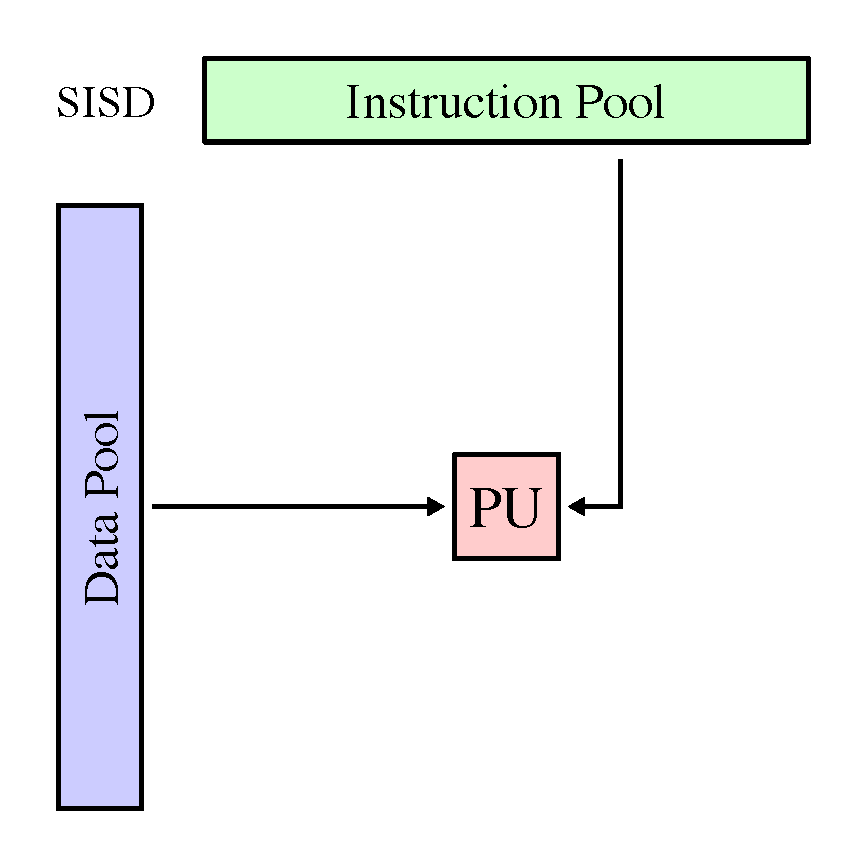
\includegraphics[width=1.\textwidth]{figures/rp/SISD}
		\caption{SISD}
	\end{subfigure}
	\begin{subfigure}[b]{0.245\thewidth}
		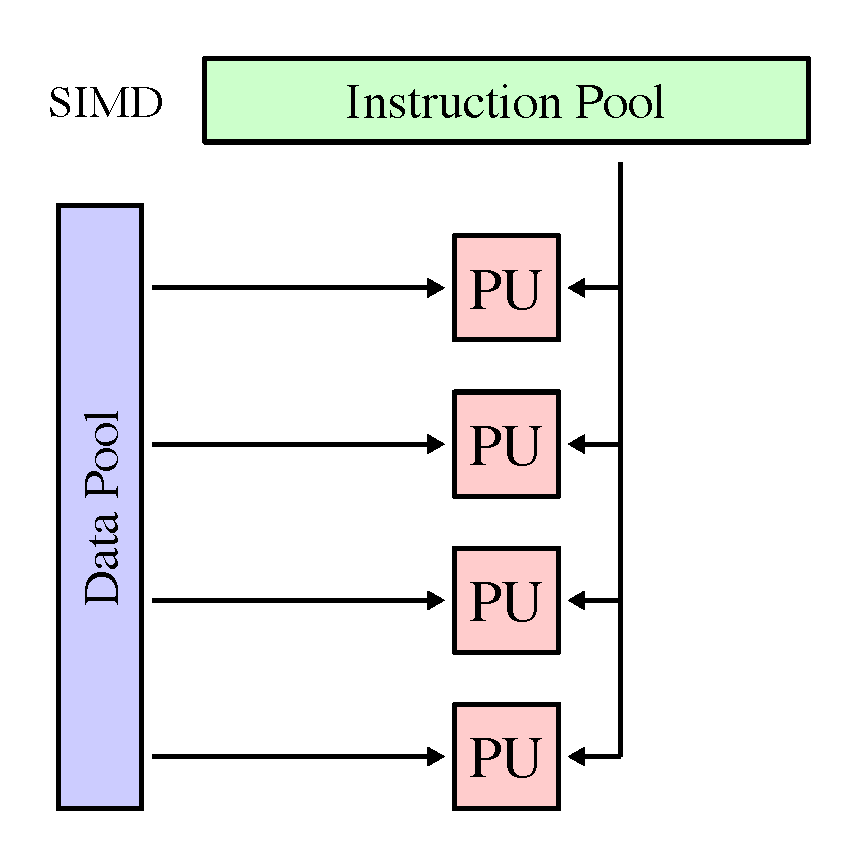
\includegraphics[width=1.\textwidth]{figures/rp/SIMD}
		\caption{SIMD}
	\end{subfigure}
	\begin{subfigure}[b]{0.245\thewidth}
		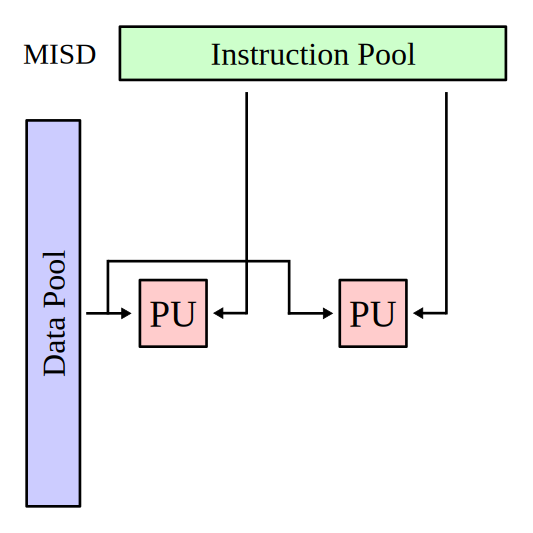
\includegraphics[width=1.\textwidth]{figures/rp/MISD}
		\caption{MISD}
	\end{subfigure}
	\begin{subfigure}[b]{0.245\thewidth}
		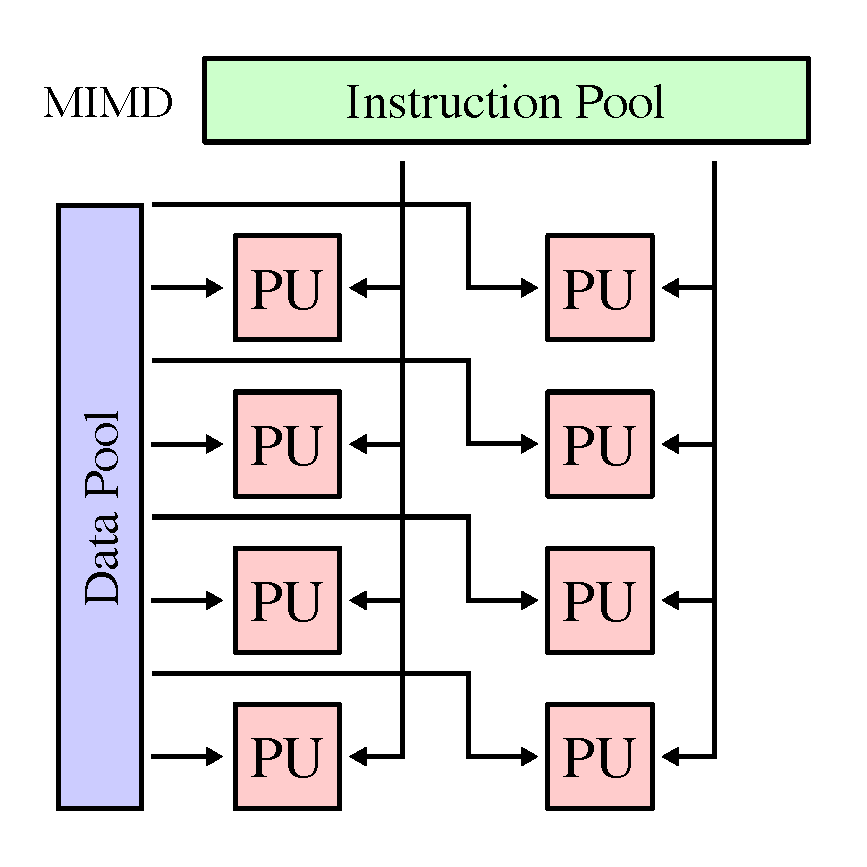
\includegraphics[width=1.\textwidth]{figures/rp/MIMD}
		\caption{MIMD}
	\end{subfigure}
\caption{弗林分类法的四种处理器,弗林分类法用来描述处理器架构中数据流和指令流之间的关系,架构类型图片来自Cburnett)}
\label{f:rp-flynn}
\end{fullwidth}
\end{figure}

绝大多数标准串行程序设计遵循的都是单指令单数据(Single instruction stream, single data stream,SISD)\index{单指令单数据single instruction stream, single data stream}\index[en]{single instruction stream, single data stream单指令单数据}模型,即在任何时间点上只有一个指令流在处理一个数据项,这相当于一个单核处理器在一个时刻只能执行一个任务。当然,它可以所谓的分时机制,即在多个人物间迅速切换,达到“同时”执行多个任务的效果。

在单指令多数据(Single instruction stream, multiple data streams,SIMD)\index{单指令多数据single instruction stream, multiple data streams}\index[en]{single instruction stream, multiple data streams单指令多数据}模型中,一个指令流被并发地广播到多个处理器上,每个处理器拥有各自的数据流,如图\ref{f:rp-flynn}(b)所示。这样,在处理器内部就只需要一套逻辑来对这个指令流进行解码和执行,而无需多个指令解码通道。由于从芯片内部移除了部分硅实体,因此SIMD相对于其他系统可以做得更小,更便宜,能耗更低,并能够在更高的时钟频率下工作。

使用SIMD,实际上就是从“对一个数据点进行一个操作”变为“对一组数据进行一个操作”,由于这组数据中的每一个元素的操作是不变的,所以指令读取和解码只需要进行一次。此外,由于数据区间是有界且连续的,所以数据可以全部从内存中一次性取出,而不是一次只取一个数据项\footnote{对连续数据进行一次性读取也是图形处理器的重要特征,我们即将看到在GPU中对一个块的数据进行一次性读取,并结合使用大量的线程块来来隐藏处于读取状态的线程块。}。

\begin{shaded*}
	注意此处的SIMD架构和SIMD指令并不是一个概念,虽然它们在意义上是类似的。SIMD指令是指在传统的处理器中,其不仅支持整型,浮点型等常见数据类型进行计算,一般现代CPU还拥有另外的SIMD寄存器来支持向量操作,例如在C++中的向量操作,编译器会转化为SIMD指令,并将一个向量内的4个数据一次性读取到寄存器中,而不是每次只读取一个。
\end{shaded*}

并没有比较知名的系统属于多指令单数据(Multiple instruction streams, single data stream,MISD)\index{多指令单数据multiple instruction streams, single data stream}\index[en]{multiple instruction streams, single data stream多指令单数据}模型,提出它仅属于完整性的缘故。

在多指令多数据(Multiple instruction streams, multiple data streams,MIMD)\index{多指令多数据multiple instruction streams, multiple data streams}\index[en]{multiple instruction streams, multiple data streams多指令多数据}模型中,每个处理单元拥有自己的指令流,并且这些指令流操作自己的数据流,如图\ref{f:rp-flynn}(d)所示,绝大多数现代并行系统都属于此类型。








\section{GPU并行计算架构}
对于习惯于针对CPU进行串行编程的程序员来讲,图形处理器(Graphics Processing Unit,GPU)总是透着一层神秘的面纱,甚至对于很多程序员,他们会认为针对GPU编程学习的难度要远远大于CPU。这种印象或者体验源于GPU编程的一些特征,例如针对CPU的串行编程符合人类的逻辑思维特征,而针对GPU的编程更多的是以并行编程为主;同时串行编程模型已经非常成熟,处理器将很多特征隐藏在硬件级别,使编译器能够对并行编程进行高度抽象,所以程序员不需要去了解处理器架构的一些知识,然而针对GPU的并行编程仍然依赖于程序员对硬件知识有一定的了解(例如GPU使用受程序员托管的内存模型,而不是完全基于硬件托管的内存模型,还有数据的对齐以及内存合并等概念),才能够充分提高并行计算的效率;另外,GPU并没有独立的编程模型,它通常是和CPU一起形成一个非对等的多处理器架构,开发者需要通过CPU来调度和管理GPU设备,内存,以及管理这些设备内的各种状态,等等。

虽然本书的内容主要只是涉及GPU图形渲染管线的运用,而并不是更广义上的GPU并行编程,然而理解图形处理器架构对于真正的图形程序开发者仍然是必不可少的知识,它有助于我们更深刻地理解图形接口以及更好地运用它们。所以本节将会详细讨论GPU架构相关的各种知识,带着这些知识,我们将会在下一章更好地理解图形渲染管线。需要注意的是,本章的内容主要围绕Nvidia的GPU处理器产品进行介绍,然而大多数现代图形处理器的架构是类似的。






\subsection{为什么需要另外一个并行计算架构}
为了更好地理解GPU架构,本节不会直接给出GPU的架构,然后讲述其对应的功能,而是选择首先讲述它的来由,通过对这些客观条件的理解,能够帮助我们更好地理解GPU架构。

由前面的内容可知,多处理器架构完全能够支持并行计算,例如它将相同的程序发送至多个处理器或线程执行,并分别赋予相应的处理数据,为了支持更大的并行性,我们可以使用更多的处理器。那么这样做存在的问题是什么?

使用一般的多处理器架构来执行大规模并行计算的限制正来源于针对串行计算优化的缓存系统,由于处理器时钟和主内存读取速度之间的巨大差异导致数据读取的巨大延迟,缓存系统通过充分利用局部性原理预取指令或数据,大大减少了对数据读取导致延迟的不必要的等待,以保证串行程序的高效执行。然而,高速缓存系统的成本非常高,并且占据芯片很大的空间,操作数从主内存到ALU之间的传输需要耗费大量的电能,这些因素使得基于缓存的处理器系统很难扩张以应付大规模的并行计算。相反,从设计处理器过程的成本来讲,计算单元ALU则是很便宜的,它们能够以很高的速度运行,而消耗很小的电能并占据很少的物理硅片空间。

所以,很明显的问题是,为了满足大规模并行计算,我们需要一些新的思路来取代缓存系统的功能及作用,理解这个新系统的特点及机制是理解GPU架构的关键。




\subsection{内存结构}
GPU架构和CPU的最大不同在内存系统上,CPU为了最大限度地减少程序员对内存的关心,使用一种称为硬件托管的内存模型,在这种模型中,缓存系统自动根据局部性特征获取当前正在执行指令附近的指令以及当前正在处理数据附近的数据,并在指令将计算结果写入到寄存器之后自动将其写入到缓存系统,以及更新多处理器架构中其他处理器的缓存。所有这些操作都是硬件自动完成的,程序员完全不需要关心其中的过程。

然而我们已经知道缓存系统的成本非常高,以至于不适用于大规模的并行计算,在大规模并行计算中,程序要处理的数据集的大小通常要数倍于一般的串行程序,我们根本不可能通过扩展缓存系统来满足大规模计算的需求,那样将导致巨大的成本。并且并行程序通常有数千个线程同时运行,大多数线程之间都是独立的,如果每个线程的中间计算结果都需要写回缓存甚至主内存,这也将是一笔巨大的浪费。

\begin{figure}
	\includegraphics[width=1.0\textwidth]{figures/rp/sm}
	\caption{NVIDIA系列GPU的内存结构,它包含寄存器,共享内存,常量/纹理内存以及全局内存。与CPU的基于硬件的缓存模型不同的是,GPU使用的是基于程序托管的内存模型,即数据的存放位置可以由程序来控制}
	\label{f:rp-sm}
\end{figure}

所以,GPU使用的是一种称为程序托管的内存模型,即数据的存放地点由程序员决定,因此它要求程序员需要对GPU内存结构有一定的了解。然而,由于GPU硬件不包含自动完成数据替换的逻辑,因此它也可以减少一部分芯片的面积以及能耗以容纳更多的计算单元。

图\ref{f:rp-sm}表示的是一个GPU内的内存结构,其中流处理器族(Stream multiprocessor,SM)\index{流处理器族stream multiprocessor}\index[en]{stream multiprocessor流处理器族}相当于一个CPU核,每个SM内部有多个流处理器(Stream processor,SP)\index{流处理器stream processor}\index[en]{stream processor流处理器},每个SP用于执行并行计算中的一个独立的线程,我们将在后面详细讲述这些概念。GPU中的内存分为4种:寄存器,共享内存,常量/纹理内存以及全局内存,每种存储类型的带宽和延迟是不同的,如表\ref{t:rp-gpu-memory}所示。

\begin{table}
\caption{GPU中不同存储类型的带宽和延迟时间}
\label{t:rp-gpu-memory}

\begin{tabular}{p{0.19\textwidth}|p{0.19\textwidth}|p{0.19\textwidth}|p{0.19\textwidth}|p{0.19\textwidth}}
\hline 
   存储类型&寄存器&共享内存&纹理/常量内存&全局内存  \\
    \hline  
 带宽&约8TB/s&约1.5TB/s&约200MB/s&约200MB/s\\
 延迟&1个周期&1-32个周期&400-600个周期&400-600个周期\\
 \hline 
\end{tabular}
\end{table}







\subsubsection{全局内存}
图形处理器又称为加速卡,它是计算机系统的一种附属设备,它不能独立运行,必须借助于CPU才能发挥作用。所以通常一个GPU应用程序包含一个CPU宿主程序,以及一些GPU内核函数,当程序运行时,宿主程序将这些GPU内核函数指令及相关的数据分发到GPU设备上计算,然后从GPU内存中取回计算结果。

GPU拥有自己独立的内存,所以宿主程序需要将数据从CPU传输到GPU以进行计算。通常GPU设备都是通过PCI-E(Peripheral Communications Interconnect Express)总线与处理器相连,如图\ref{f:rp-pci-e}所示,目前PCI-E 3.0的传输速率为8GB/s。PCI-E是全双工总线,这意味着数据的传入和传出可以同时进行并享有同样的速率,也就是说我们在以8GB/s的速度向GPU卡传送数据的同时,还能够以8GB/s的速度从GPU卡接受数据\footnote{然而实际上数据在CPU和GPU内存之间的传输还会经历一些低速的前端总线,所以实际上并不能达到8GB/s这么高的速率。不过Nvidia在其最新的Pascal处理器架构\cite{a:PascalArchitectureWhitepaper}中使用了一种新的直连技术Nvlink,它可以使GPU之间通过Nvlink而不是PCI-E连接,其可以提高GPU-GPU之间高达160GB/s的传输速度。如果处理器本身支持Nvlink技术(例如IBM的POWER8处理器),其还可以提供相同的CPU-GPU之间的传输速度。}。然而,这并不意味着如果不接受数据,我们就可以以16GB/s的速度向GPU卡传送数据。

\begin{figure}
\sidecaption
	\includegraphics[width=.65\textwidth]{figures/rp/pci-e}
	\caption{在一般的处理器架构中,GPU通过PCI-E总线与CPU联通}
	\label{f:rp-pci-e}
\end{figure}

GPU中的主内存称为全局内存,这是因为GPU和CPU都可以对其进行写操作。宿主程序要想在GPU上执行计算,首先将CPU中的数据和指令通过PCI-E总线传输至GPU的全局内存中,然后GPU中的各个内核线程从全局内存中读取数据并执行计算,然后将计算结果写回到全局内存,宿主程序再从GPU全局内存中读取数据回CPU中。例如图形渲染管线中的顶点数组,纹理数据等,即是通过OpenGL等图形接口将CPU中的顶点数据传输到GPU全局内存中,只不过在图形接口中通常还会做一些数据的格式转换(例如归一化)。

由于并行计算涉及巨大的数据集,这些数据从CPU到GPU全局内存之间的传输,以及全局内存到GPU内核函数的的寄存器之间的传输都会产生大量的延迟,所以在GPU中可以使用一种比较高级的流传输的模型来使传输数据和内核函数的执行重叠进行,参见本章后面的内容。

全局内存是GPU中内核函数访问最慢的内存,由于GPU架构使用程序托管的内存模型,所以内核函数可以选择不需要将每个变量的中间结果都写回到全局内存,这些中间数据可以保存在内核函数所在的执行单元本地,而等到内核函数执行完毕时才将本地的数据写回到全局内存,这大大节省了数据在全局内存和内核函数之间的不必要的传输时间;此外,一个线程束的线程对全局内存连续地址的访问还会涉及合并,这些内容将在本章后面描述。





\subsubsection{常量/纹理内存}
对于并行计算,每个线程使用的数据大都是相互独立的,例如对一个数组进行操作,每个线程分别读取数组中的一个元素进行相关的计算,线程$i$通常不需要数组中除$i$之外的元素数据。这样的数据可以直接存放在全局内存中,线程执行时内核函数直接(不经过缓存系统)向全局内存请求,如果相邻线程请求的数据地址是连续的,它们可以被合并使其只有一次内存请求,再结合后面的延迟隐藏技术,可以提供比较高的计算效率。

然而,对于另外少量可以被多个线程随机访问的数据,并且多个线程可以访问同一个数据,这样的数据使用全局内存存储,然后直接被内核函数访问则效率不高。所以GPU提供另外一种内存结构用来存储这类可以被随机访问的数据。

常量以及纹理内存其实只是全局内存的一中虚拟地址形式,GPU并没有特殊保留的常量/纹理内存,但是常量/纹理内存能够提供高速缓存。此外常量内存和纹理内存都是只读内存。

如图\ref{f:rp-sm}所示,常量内存可以被缓存到常量内存缓存存储器,而纹理内存可以被缓存到纹理内存缓存存储器,这些缓存存储器通常是L1级缓存,可以提供较全局内存更快的访问速度。然而由于所有缓存系统都是利用数据的局部性原理,所以它要求所有线程对数据的访问可以局部化到一个缓存的大小。例如一个64KB的常量大小以及一个8KB的常量缓存大小,这意味着可缓存的内存大小比为8:1,如果能够将访问的数据包含或局部化到常量内存中一个8KB大小的块中,那么程序将获得很高的性能。否则,对于非均匀的常量内存访问,如果缓存没有命中所需的数据,将导致N次对全局内存的访问,而不但是从常量缓存上获取数据。因此,对于那些数据不太集中或数据利用率不高的内存访问,尽量不要使用常量内存。

此外,对于纹理内存,它好提供基于硬件的线性插值功能。对于第一章讲述的纹理的放大和缩小操作,硬件会基于给定的纹理坐标值获取该纹素(texel)附近的多个纹素值,然后基于这些纹素值进行插值计算。对于一维数组来讲,它使用简单的线性插值,对于二维数组和三维数组,分别可以支持硬件级双线性插值和三线性插值。这样就使得渲染管线中的贴图可以高速处理。

纹理的另一个比较实用的特性是其可以根据数组索引自动处理边界条件,我们可以在数组边界按照环绕方式或夹取方式来对纹理数组进行处理。这一点非常有用,因为通常情况下它不需要通过嵌入特殊的边缘处理代码就可以对所有元素进行处理。而特殊情况下的代码处理通常会导致线程分支的产生,参见本章后面线程分支处理相关的内容。






\subsubsection{共享缓存}
由后面图形学处理器架构一节的内容可知,内核函数的多个线程会分配到多个SM上执行,据此我们可以对并行计算处理的数据进行一定的划分成多个处理子块,在每个子块内部的多个线程可以共享一些局部数据。如图\ref{f:rp-sm}所示,这些单个SM内部的局部数据不需要通过缓慢的全局内存进行存储和读取,它们可以被存储在一个SM内部的共享内存当中。共享内存实际上是一个位于SM附近的L1高速缓存,它的延迟极低,大约有1.5TB/s的带宽,远远高于全局内存,但是它的速度大约只有寄存器的1/10。

为了提供更高的带宽,共享内存使用的是基于存储器切换的架构(bank-switched architecture),它将共享内存平均分成多个相同尺寸的内存模块,称为存储体(banks),这些存储体内的内存可以被同时使用。任何对共享内存读或者写的操作可以均分到$n$个不同的存储体地址的都可以同时进行,使其可以提供相对于单个内存模块$n$倍的带宽。

例如费米架构的设备上有32个存储体,无论有多少个线程发起操作,每个存储体每个周期只执行一次操作,因此如果一个线程束(参见后面的内容)中的每个线程访问一个存储体,那么所有线程的操作都可以在一个周期内同时执行。此时无须顺序地访问,因为每个线程访问的存储体在共享内存中都是独立的,互不影响。如图\ref{f:rp-shared-memory}中上面的顺序访问,或者随机但是每个线程访问不同的存储体,这两种情况都可以同时执行。

\begin{figure}
\begin{fullwidth}
	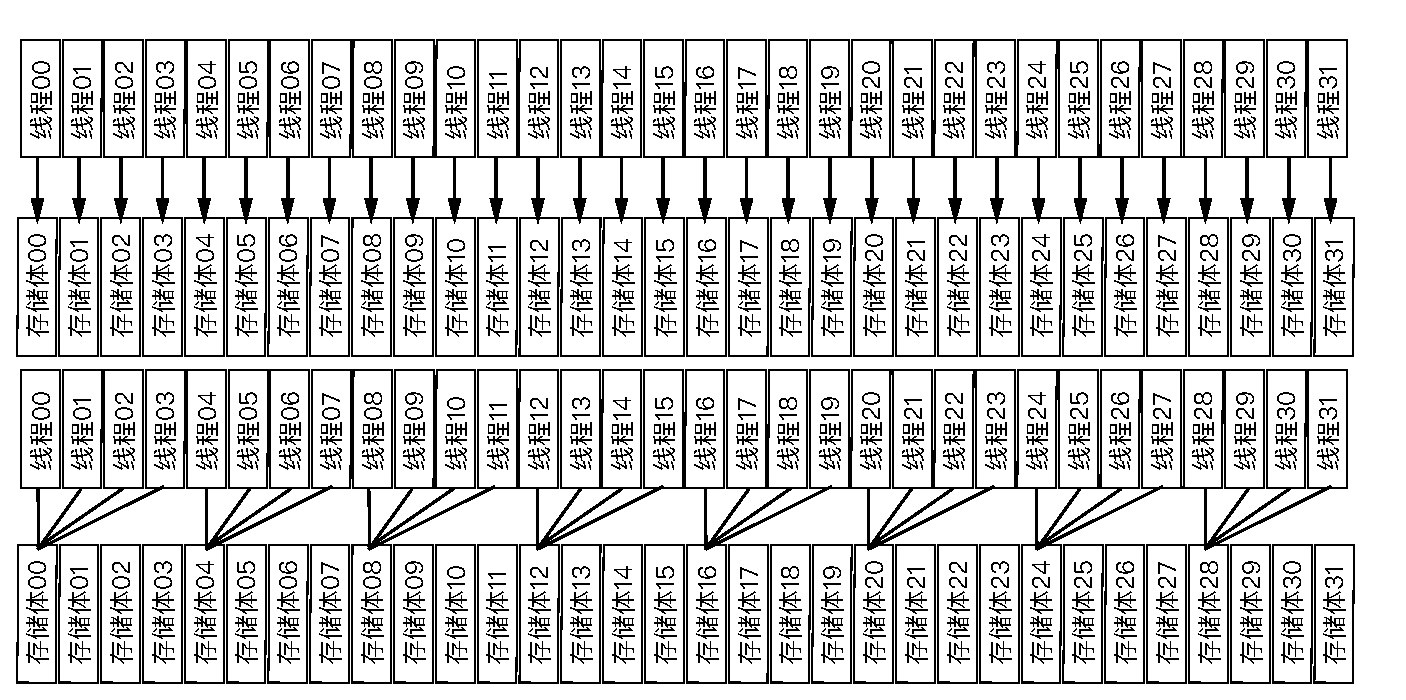
\includegraphics[width=1.0\thewidth]{figures/rp/shared-memory}
	\caption{共享内存被平均分配到32个存储体上,每个存储体在同一个周期内可以独同时被访问。上面的顺序访问(或者随机独立访问)可以被同时执行,然而下面多个线程读取同一个存储体将导致存储体冲突}
	\label{f:rp-shared-memory}
\end{fullwidth}
\end{figure}

此外,当线程束中所有线程同时访问相同地址的存储体时,会触发一个广播机制到线程束的每个线程,其他情况则将导致存储体冲突(bank conflicts)\index{存储体冲突bank conflicts}\index[en]{bank conflicts存储体冲突},例如一个线程束中只有一部分多个线程访问同一个存储体则需要排队,此时当一个线程访问共享内存时,线程束中的其他线程将被阻塞闲置,并且此时并不会导致后面会讲述的延迟隐藏机制使处理器切换到其他线程执行。所有使用共享内存需要小心处理存储体冲突。





\subsubsection{寄存器}
与CPU架构不同的是,GPU的每个SM拥有一个巨大的寄存器文件,它通常包含上千个寄存器,例如在费米架构的设备上,每个SM拥有32KB的寄存器空间,这些寄存器平均分配到每个SP,根据线程的数量,每个线程可以使用几个到几十个寄存器。寄存器的读取速度是最快的,约相当于1个GPU时钟周期。

之所以使用数量巨大的寄存器,其一是因为即将在下一节讨论的延迟隐藏的需求,其二是因为GPU寄存器的特征。GPU中的寄存器与CPU中的寄存器是不同的,在CPU中,指令执行完后写入寄存器中的数据会被自动写入到缓存中去,然后缓存系统会广播更新多处理器架构中其他处理器的缓存,以及将数据写入到主内存。然而GPU并不会这么做,写入到寄存器中的数据会一直停留在该寄存器中,直到有新的数据写入或者当前线程执行完毕自动退出,寄存器数据被重置。这就是称为程序托管的内存模型的原因,程序员指定一个变量的内存类型,即是指定了其数据的存放位置,处理器不会自动变更这个位置。

这样做的原因是什么呢?由于GPU可能同时处理上千个相同指令的线程,每个线程在执行过程中某些中间计算结果只供自己所在的线程使用,所以它完全没有必要写入到全局内存中去。在一个GPU内核函数中,每个本地变量都会自动存储到寄存器,这些变量不会被自动更新到全局内存,只有当该线程计算结束,或者某些中间过程需要将数据写入到全局的时候,才将寄存器中的数据赋值给全局内存变量,这样将大大节省不必要的数据在内存中的流通,例如在一个OpenGL的着色器程序中,通常只有最后才会将结果写回到全局内存,这些值可能是顶点着色器中执行过变换的坐标值,或者像素着色器中计算出的颜色值。但同时这也需要每个线程拥有大量的寄存器,因为每个本地变量都需要占用一个寄存器。

此外,每个SP线程都拥有自己独立的寄存器还可以避免线程切换时导致的寄存器数据的换进换出。在CPU中,当一个线程处于延迟等待状态时,处理器会切换到其他准备好的线程进行执行以隐藏延迟,GPU同样使用了延迟隐藏技术,如下一节所述,并且它更是将延迟隐藏技术发挥到极致,而大量的寄存器导致GPU线程切换的成本几乎为0。






\subsection{图形处理器架构}
本节我们以Nvidia当前的旗舰消费级开普勒(Kepler,\cite{a:NVIDIAsNextGenerationCUDATMComputeArchitecture:KeplerTMGK110/210})架构为例讨论图形处理器的架构,如图\ref{f:rp-kepler}所示(Nvidia下一代图形处理器架构为Pascal\cite{a:PascalArchitectureWhitepaper})。

\begin{figure}
	\begin{fullwidth}
		\includegraphics[width=1.0\thewidth]{figures/rp/kepler}
		\caption{Nvidia开普勒架构的GK110/210系列处理器}
		\label{f:rp-kepler}
	\end{fullwidth}
\end{figure}

GPU通常是和CPU组成一个非对等的计算环境,其中CPU充当宿主程序,并负责计算一般的串行程序,而另一些计算密集,具有高度并行性特征的程序则被发送到GPU执行。这些仅在GPU上执行的并行计算程序称为内核函数(kernels)\index{内核函数kernels}\index[en]{kernels内核函数},CPU负责在GPU上分配内存,并将内核函数以及相关数据发送到GPU内存,GPU的计算单元从这些内存获取数据并进行大规模的并行计算,最后CPU从GPU内存中取回计算结果。

GPU实际上是一个SM阵列,这就是GPU具有可扩展性的关键因素,如果向设备中增加更多的SM,GPU就可以在同一时刻处理更多的任务,例如使用开普勒架构的GK110/210系列处理器拥有15个SMX(注意,由于开普勒较上一代处理器有很大改进\footnote{其中比较重要的调整是将之前费米架构中每个线程每个时钟周期内执行2条指令,改为每个时钟周期执行一条命令。这虽然减少了一半的吞吐量,但是开普勒架构拥有更多的内核,以及减少“时钟频率”带来的能量消耗等问题,开普勒架构较前代仍有大幅性能的提升。},所以Nvidia称其新的流处理器族为SMX而不是SM)。

每个SMX中包含若干个流处理器SP以及其他一些关键部件,如寄存器,共享内存,硬件支持的特别计算单元(Special function units,SPU)\index{特别计算单元special function units}\index[en]{special function units特别计算单元}等。在每个SMX内执行的是相同的指令,因此它们只需要一次指令获取,然后广播到SMX内的各个SP,所以SMX使用的是SIMD架构模型,但是Nvidia更趋向于称之为SPMD,即单程序多数据(Single Program Multiple Data)\index{单程序多数据Single Program Multiple Data}\index[en]{Single Program Multiple Data单程序多数据}。

开普勒架构的GK110/210均提供每个SMX内部192个SP,所有理想情况下每个SP每个时钟周期可以同时执行192个线程,这使得GK110/210均可以提供的每秒浮点数计算次数(Floating Point Operations per Second,Flops或Flop/s)\index{每秒浮点数计算次数Floating Point Operations per Second}\index[en]{Floating Point Operations per Second每秒浮点数计算次数}高达1TFlop/s(1T=$10^{12}$)。

当然,图形处理器的硬件架构还包括很多知识,然而本书并不是一本描述并行计算的书籍,我们讨论处理器架构的目的是用来帮助我们理解并行程序的执行以及它的一些特性,然而我们并不需要理解它内部到底怎么执行,感兴趣的读者可以阅读\cite{a:NVIDIAsNextGenerationCUDATMComputeArchitecture:KeplerTMGK110/210,a:PascalArchitectureWhitepaper,a:CUDACPROGRAMMINGGUIDE}等以了解更多关于并行计算的知识。






\subsection{延迟隐藏}\label{sec-rp-latency}
由于处理器时钟频率和主内存读取速度以及带宽的差异,导致数据从主内存传输到处理器计算单元的过程存在很大的延迟,例如全局内存的访问高达400-600个时钟周期。

为了克服这种延迟,一些技术通过一些辅助手段来“隐藏”这种延迟,这种技术称为延迟隐藏(Latency hiding)\index{延迟隐藏latency hiding}\index[en]{latency hiding延迟隐藏}。在CPU中主要使用缓存来隐藏延迟,缓存系统一次性读取一个缓存行的数据,如果指令之间处理的数据是连续的,那么同一缓存行内的后续的数据的延迟将被隐藏;另一方面,如果数据来自于下一个缓存行,则可以使用预取技术来提前缓存相邻的缓存行来达到延迟隐藏。

然而,这种基于硬件托管的缓存系统并不适于大规模的并行计算,由于硬件托管的缓存系统会自动将所有写入寄存器的值更新到缓存系统以及主内存中,而并行计算线程之间独立性比较高,大部分中间计算结果都不需要写回缓存中去,所以GPU使用的是程序托管的内存模型。并且,GPU中虽然仍然会使用缓存,然而GPU的缓存系统主要面向一些共享数据(部分线程之间或全部线程之间共享),对于大部分独立的线程数据,GPU使用另一种方式来隐藏延迟。

回想前面讲述单个处理器的多线程技术,当一个线程处于延迟状态时,处理器自动切换到其他处于等待执行状态的线程进行执行,这样通过使用多于处理器能够处理个数的线程数目,内存读取的延迟也能够在一定程度上被隐藏。

GPU正是将这种延迟隐藏技术发挥到了极致,要放大这种技术的隐藏作用,有两个方面可以改进,其一是使用能够容纳更多的等待线程。在GK210/110架构中,虽然每个SMX只有192个SP,但是每个SMX可以分配最多高达2048个线程,即是说当每个时钟周期有192个线程在执行计算的时候,还可以有将近2000个线程正在从内存中获取数据,这样通过大量的线程就使得大部分线程的内存获取的延迟被隐藏了。

CPU多线程技术的另一个瓶颈来源于少量的寄存器,虽然每个时钟周期可以容纳多个线程处于延迟状态,但是由于寄存器数量的不足,这些线程的数据被放入在缓存系统当中,使得每次切换线程时都需要寄存器数据的换进换出,因此执行多线程就需要大量的延迟。GPU同样用到上下文切换的概念,但是它拥有数量众多的寄存器,它致力于为每一个线程都分配真实的寄存器,哪怕是处于等待状态的线程,这正是它隐藏延迟的秘密所在,因此,一次上下文调换只需要重新执行另一个寄存器组。在GK110架构中,每个SMX有65 536个32为的寄存器,GK210更是高达131 072个32位寄存器。使得每个线程可以拥有多达32(65 536/2048)个以上寄存器可用。

此外,利用这种延迟隐藏技术,还可以实现内核的执行与从CPU到GPU内存的传输重叠进行。如图\ref{f:rp-streaming}所示,如果内核函数直接从CPU而不是从GPU的全局内存获取数据,就可以不需要等待所有数据都传输至GPU之后再开始执行内核函数的计算。由于并行计算提成涉及大量的数据集,这种重叠技术可以使得GPU的利用率更高(不需要在CPU向GPU传输大量数据集的时候空闲等待)。

\begin{figure}
	\includegraphics[width=1.\textwidth]{figures/rp/streaming}
	\caption{内核执行与内核传输重叠进行}
	\label{f:rp-streaming}
\end{figure}




\subsection{全局内存访问的合并}
并行计算的性能,还可以得益于其程序和数据的一致性,这种一致性越高,能够实现的吞吐率就越高,反之数据的存储越发散,则将导致更低的吞吐率。所以,除了需要管理内核函数变量的内存位置,并行计算的另一个难点还在于程序员需要去精心设计全局内存数据的布局。

GPU使用一种称为内存合并(Memory coalescing)\index{内存合并memory coalescing}\index[en]{memory coalescing内存合并}的技术来充分利用并行程序的数据连续性。当连续的线程向全局内存发起数据请求,并且请求的内存块是连续对齐时,这些线程的多个内存请求会被合并成一次请求,然后一次性返回所有数据。一般可以返回整个线程束所需要的数据,如图\ref{f:rp-coalescing}所示。SMX中的线程每32个会被组成一个线程束(Thread wrap)\index{线程束thread wrap}\index[en]{thread wrap线程束},每个线程束内的线程会被保证同步执行。由于一个存储事务是需要一定开支的,内存合并使得多个线程的内存请求只需要一个存储事务即可解决问题。

\begin{figure}
	\begin{fullwidth}
		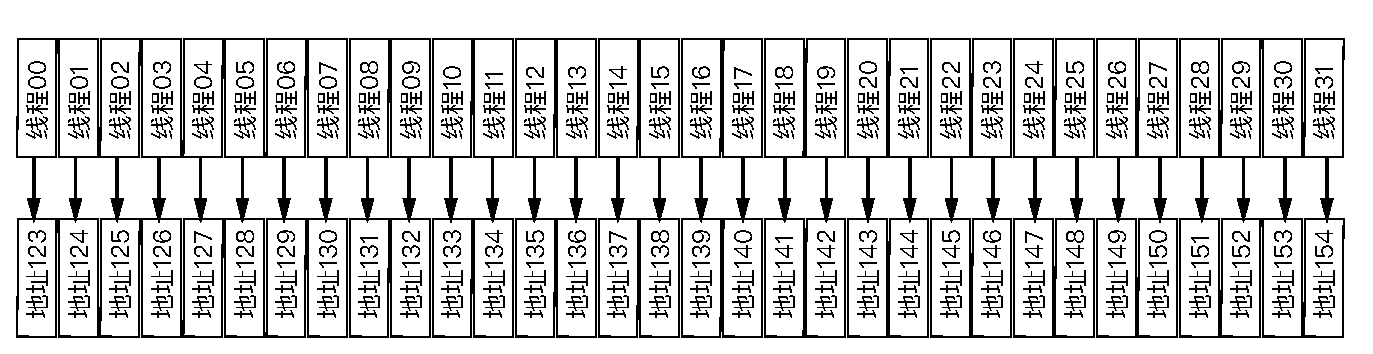
\includegraphics[width=1.0\thewidth]{figures/rp/coalescing}
		\caption{一个线程束内相邻线程对相邻连续对齐的内存的读取将会被合并成一次读取,大大减少存储相关事务的开支}
		\label{f:rp-coalescing}
	\end{fullwidth}
\end{figure}

内存会基于线程束的方式进行合并,内存合并事务大小支持32,64以及128-bytes,分别表示线程束中每个线程以1,2以及4个bytes为单位读取数据。全局内存支持单个指令读或写的请求的内存大小为1, 2, 4, 8, 或者 16 bytes,要想获得内存合并,每个线程访问的数据必须基于这些基础数据对齐的,否则将不能获得内存合并的好处。所谓对齐(align),即是指每次指令获取的数据所占内存大小是和内存系统支持的存取单位一致的,例如一个数据所占内存大小为10bytes,将导致返回一个16bytes的数据,这个数据类型就是没有对齐的。

所有内置类型如char, short, int, long, longlong, float以及双精度的float2 和 float4都是自动对齐的,对于用户自定义的数据类型,其可以使用对齐标识符\_\_align\_\_ 进行强制对齐(但这样将导致一些为定义的数据浪费内存,所以通常我们应该精心设计自定义类型以充分利用内存合并以及内存的占用),如:

\begin{lstlisting}
struct __align__(8) {
    float x;
    float y; 
};
\end{lstlisting}

或者:
\begin{lstlisting}
struct __align__(16) {
	float x;
	float y;
	float z; 
};
\end{lstlisting}






\subsubsection{分~~支}
最后我们要讨论的是条件分支指令,传统的CPU的目标是执行串行代码,它们包含了一些特殊硬件,例如分支预测单元,多级缓存等,所有这些都是针对串行代码的执行;但GPU并不是为执行串行代码而设计的,为了高效执行大量的并行计算,GPU并没有像CPU那么复杂的硬件实现的分支预测功能,同前面的变量内存位置分配,数据的连续对齐一样,条件分支同样需要程序员小心地处理。

对于分支指令,GPU在执行完分支结构的一个分支后会接着执行另一个分支,对不满足条件的分支,GPU在执行这段代码的时候会将它们设置成为激活状态,当这块代码执行完毕之后,GPU继续执行另一分支。这种机制是由于每个SMX内的每个线程束每次只获取一条指令,它不能同时获取条件为真和条件为假两条指令。

这样导致的结果就是,当程序中包含分支指令时,如果在一个线程束内的分支分布是不连续的,例如图\ref{f:rp-branching}(b)所示,则将导致在处理分支的时候部分线程处于空闲状态,不能充分利用GPU的计算资源。更糟糕的是,这种由于分支导致的线程并不会导致处理器将计算资源切换到其他线程束执行,即是说,由于分支导致的部分线程的闲置并不能算作线程阻塞,只有内存读取的延迟才能促使线程切换。

\begin{figure}
\begin{fullwidth}
	\begin{subfigure}[b]{0.24\thewidth}
		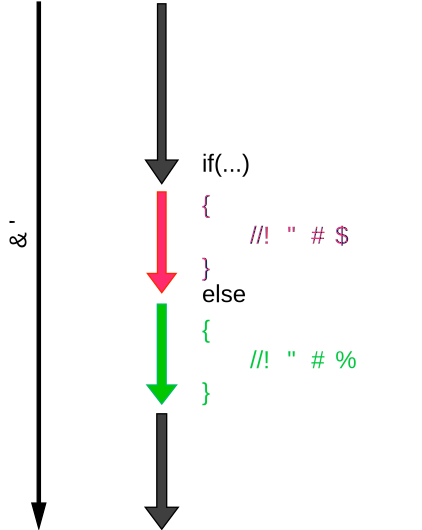
\includegraphics[width=1.\textwidth]{figures/rp/branching-1}
		\caption{条件分支指令}
	\end{subfigure}
	\begin{subfigure}[b]{0.24\thewidth}
		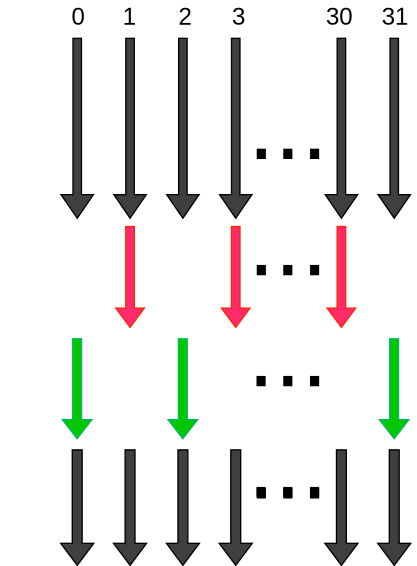
\includegraphics[width=1.\textwidth]{figures/rp/branching-2}
		\caption{分支分布不连续}
	\end{subfigure}
	\begin{subfigure}[b]{0.51\thewidth}
		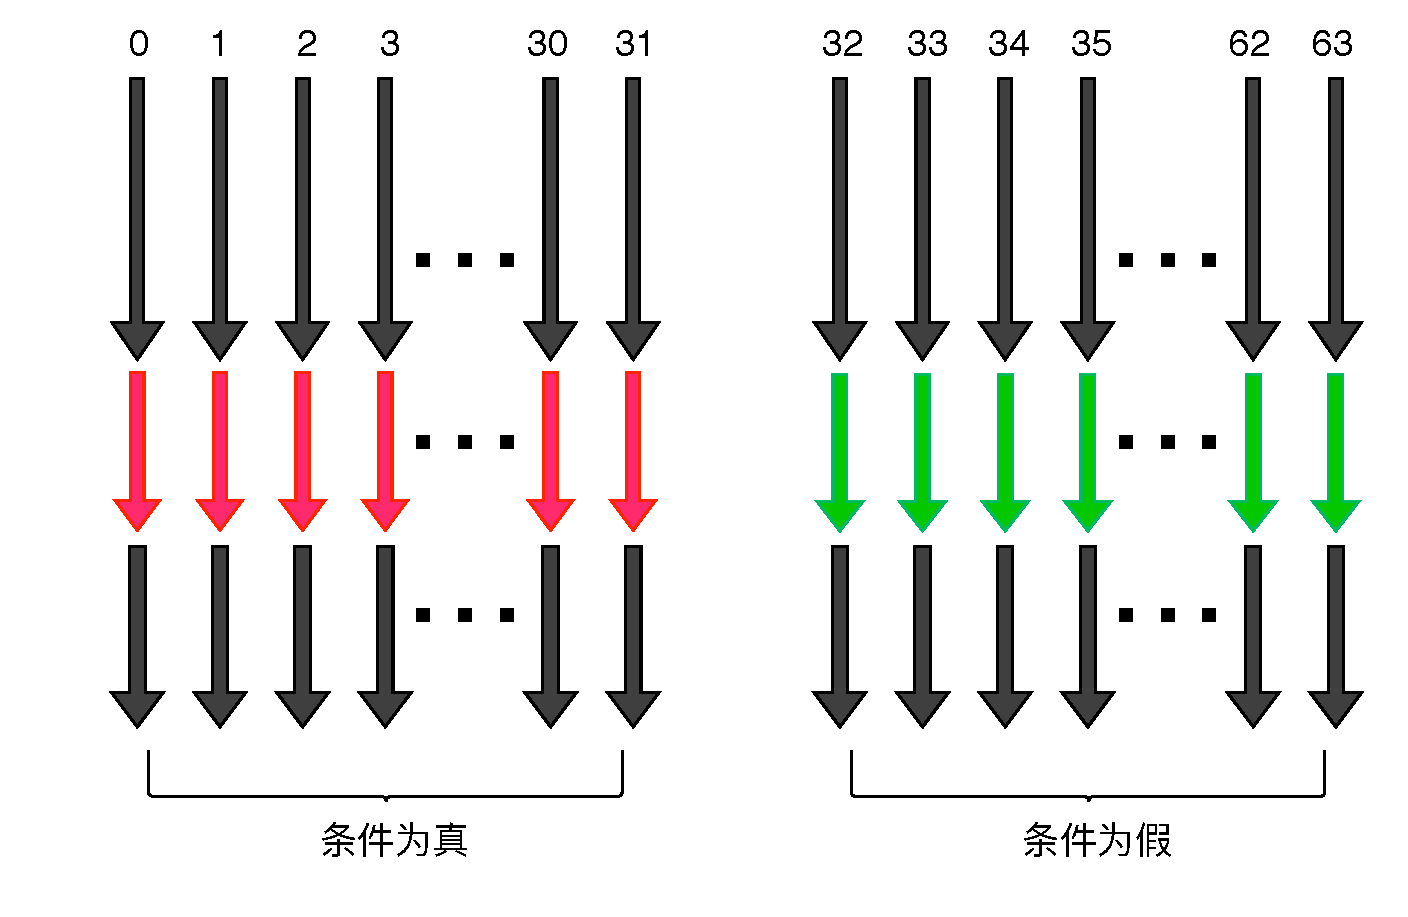
\includegraphics[width=1.\textwidth]{figures/rp/branching-3}
		\caption{连续的分支分布}
	\end{subfigure}
\caption{GPU并没有复杂的分支预测单元,这是由于其SIMD架构特性决定的,SIMD在一定的数据内只获取指令一次,所以不连续的分支将导致资源闲置,但是连续的分支分布则可以避免这种闲置}
\label{f:rp-branching}
\end{fullwidth}
\end{figure}

不过在指令的层面,硬件的调度是基于半个线程束,只要我们能够将半个线程束中连续的16个线程束划分到同一分支中,那么硬件就能同时执行分支结构的两个不同条件的分支块。然而这种条件非常苛刻,对于分支指令,最有效的方法是尽量保证分支的连续性,对于所有线程组成的条件数组排序,或者以某种方式的处理,使得分支能够连续排列。例如如果条件是大于某个数$n$,则可以让数组中的原始以$n$分割进行排列,左边的数全部大于$n$,而右边的数全部小于或等于$n$,这将导致分支分布比较连续,仅在分割的位置或者两端可能出现分布不连续。由于一个大型的并行计算常常有上万的线程,因此这种小小的优化也可以带来一定的性能提升,分支分布连续的指令执行如图\ref{f:rp-branching}(c)所示。












\begin{comment}

\section{PS4及XBox One图形硬件参数剖析}


The first is that GPU memory subsystems are fast. Seriously fast. A Core i7 2600K will hit maybe 19 GB/s memory bandwidth – on a good day. With tail wind. Downhill. A GeForce GTX 480, on the other hand, has a total memory bandwidth of close to 180 GB/s – nearly an order of magnitude difference! Whoa.

The second is that GPU memory subsystems are slow. Seriously slow. A cache miss to main memory on a Nehalem (first-generation Core i7) takes about 140 cycles if you multiply the memory latency as given by AnandTech by the clock rate. The GeForce GTX 480 I mentioned previously has a memory access latency of 400-800 clocks. So let’s just say that, measured in cycles, the GeForce GTX 480 has a bit more than 4x the average memory latency of a Core i7. Except that Core i7 I just mentioned is clocked at 2.93GHz, whereas GTX 480 shader clock is 1.4 GHz – that’s it, another 2x right there. Woops – again, nearly an order of magnitude difference! Wait, something funny is going on here. My common sense is tingling. This must be one of those trade-offs I keep hearing about in the news!

Yep – GPUs get a massive increase in bandwidth, but they pay for it with a massive increase in latency (and, it turns out, a sizable hit in power draw too, but that’s beyond the scope of this article). This is part of a general pattern – GPUs are all about throughput over latency; don’t wait for results that aren’t there yet, do something else instead!
\end{comment}
